\documentclass[10pt,  english, makeidx, a4paper, titlepage, oneside]{book}
\usepackage[utf8]{inputenc}
\usepackage{caption}
\usepackage{subcaption}
\usepackage[english]{babel}
\usepackage[utf8]{inputenc}
\usepackage{fancyhdr}
\usepackage{makeidx}
\usepackage{titlesec}
\usepackage{listings}
\usepackage{hyperref}%package per fare i riferimenti
\usepackage{appendix}

\hypersetup{hidelinks}%Questo permette di fare i collegamenti trasparenti senza riga rossa sopra
\usepackage{graphicx}
\usepackage{tikz-timing}[2014/10/29]
\usetikztiminglibrary[rising arrows]{clockarrows} 
\usepackage{xparse} % NewDocumentCommand, IfValueTF, IFBooleanTF
\usepackage{float}
\usepackage{multirow}
\usepackage{verbatim}
\usepackage{caption}
\usepackage{subcaption}
\usepackage{geometry}
\usepackage[cache=false]{minted}
\usepackage{wrapfig}
\usepackage{booktabs}


\textwidth 16cm
\textheight 23cm
\topmargin -1cm
\oddsidemargin 0cm
\linespread{1.1}

\titleformat{\chapter}[display]     %formattazione testa dei chapter della Graziano
{\normalfont\Large\filcenter\sffamily}
{\titlerule[0.5pt]%
\vspace{1pt}
\titlerule
\vspace{1pc}
\LARGE\MakeUppercase{\chaptertitlename} \thechapter
}
{1pc}
{\titlerule
\vspace{1pc}
\Huge}

\pagestyle{fancy}
\lhead{}
\chead{Integrated System Architecture}
\lfoot{}
\cfoot{}
\rfoot{}
\rhead{\thepage}

\begin{document}

\frontmatter
\begin{titlepage}
\vspace{0cm}
\centerline{

\includegraphics[width=3cm]{pics/logopoli}} 
\vspace{0.5cm}
\centerline{\LARGE Politecnico di Torino}
\vspace{2.5cm}
\centerline{\huge\sf Integrated System Architecture}
\vspace{1cm}
\centerline{\Huge\sf A RISC-V Processor: Design \& Development}
\bigskip
\centerline{\huge\sf Project Report}
\vspace{2cm}
\centerline{\Large Master's Degree in Electronic Engineering}
\bigskip
\vspace{2.5cm}
%%%%%%%%%%%%%%%%%%%%%%%%%%%%%%%%%%%%%%%%%%%%%%%%%%%%%%
%
\centerline{\large Referents: Prof. Martina Maurizio, Prof. Masera Guido}
\bigskip
\vspace{1cm}
%
%%%%%%%%%%%%%%%%%%%%%%%%%%%%%%%%%%%%%%%%%%%%%%%%%%%%%%
% GROUP
% Change the name of your group below
%
%
%%%%%%%%%%%%%%%%%%%%%%%%%%%%%%%%%%%%%%%%%%%%%%%%%%%%%%
% AUTHORS
% Change the name of the Group participants here
%
\centerline{\Large \textbf{Rovere Enrico, Santoro Dino, Sarda Giuseppe, Sartoni Sandro}}
%
%%%%%%%%%%%%%%%%%%%%%%%%%%%%%%%%%%%%%%%%%%%%%%%%%%%%%%
\vspace{1.5cm}
\centerline{\large \today}
\end{titlepage}

\tableofcontents

\newpage

\subsection*{Introduction}
The aim of the presented work is modeling a processor core compliant with the RISC-V specifications as of the official website\footnote{RISCV Specifications Website: https://riscv.org/specifications/}.
What the group did was choose a subset of the RISC-V Instruction Set Architecture (ISA) and produce the HDL modelling the resultant architecture. 

The RISC-V ISA is modular, meaning that, given a defined and fixed word size (32 bits in this case), a given core must support only the \textbf{[I]} - \textbf{Integer} subset. Of course, the architecture may be more complex and include optional \textit{extensions}, like \textbf{[M]} - \textbf{Integer Multiplication and Division}, and many more. The software to be run on the device is then compiled specifying which subsets the target supports, replacing unsupported instruction with a software library.\\
%There are many different subset of instructions, as a convention they have been grouped by means of capital letters that summarize the functionalities each set implements: \textbf{I} stands for \textbf{Integer}, \textbf{M} stands for \textbf{integer Multiplication and division}, \textbf{E} stands for a subset of instructions intended for \textbf{Embedded systems} and so on. Eventually, some of these extensions may be referred to 32-bits, 64-bits or even 128-bits architectures. \newline
Since we wanted to implement an Core as general purpose as possible, we opted for the \textit{I} extension, implementing a \textbf{RV32I} architecture.
Following, the set of instructions supported:

\begin{table}[h]
    \centering
    \begin{tabular}{|c|c|c|}
        \hline
        \textbf{Mnemonics} & \textbf{Mnemonics} \\
        \hline
        add     &   lui &  lh\\
        \hline
        addi    &   suipc&  lw\\
        \hline
        sub     &    slt&   sb\\ 
        \hline
        and     &   slti &   sh\\
        \hline
        andi    &   sltu &   sw\\ % 5
        \hline
        or      &   sltiu&   lbu\\
        \hline
        ori     &   beq &   lhu\\ 
        \hline
        xor     &   bne&   mul\\
        \hline
        xori    &   bge &   mulh\\
        \hline
        sll     &   bgeu&   mulhsu\\ % 10
        \hline
        slli    &   blt  &   mulhu\\ 
        \hline
        sra     &   bltu  &   div\\
        \hline
        srai    &   jal  &   divu\\
        \hline
        srl     &   jalr  &   rem\\
        \hline
        srli    &   lb  &   remu\\ % 15
        \hline


    \end{tabular}
    \caption{Set of Instructions supported by our Core}
    \label{tab:supported_instruction}
\end{table}
Originally, the RV32I set of instructions includes some additional instructions needed for hardware threading, we decided not to support Operating Systems and keep the implementation as straightforward as possible, thus not including these instructions.
\mainmatter
\chapter{Control Unit}
\label{cu}
The Control Unit is effectively the brains of the device, manipulating data flowing through the datapath.
\section{Overview}
The group chose a "hardwired" approach for the present unit, creating a Look Up Table (LUT) of Control Words (CW) indexed by opcode and sequentially fed to the datapath control signals. Once a CW is fetched, it is progressively shifted to separate signals - \textit{cw1, cw2, cw3} - each mapped to the port it is meant to control. 
\\
Moreover, R-type and I-type instructions require decoding of their FUNC field, which determines the operation to be performed by the ALU on the operands. Therefore, the CU includes a decoding unit for this purpose, producing an \textit{ALU\_control} signal which is then fed to the ALU, delayed by an appropriate amount of clock periods.

\section{Control Hazards}
Despite the fact that this architecture employs a Forwarding Unit, described in Section \ref{fwdu}, some Read-After-Write data dependencies may not be solved at runtime, requiring a stall of the pipeline. For any hazardous pair of instructions, the possible cases are the following:
\vspace{0.5cm}
\begin{center}
    \begin{tabular}{l||c|c|c|c|c|c}
        
         & \textbf{IF} & \textbf{ID} & \textbf{EX} & \textbf{MEM} & \textbf{WB} & \textbf{Duration} \\
        \hline
        \hline
        1) \textit{any} & \multirow{2}{*}{\texttt{S}} & & & & & \multirow{2}{*}{1 clk cycle} \\
        2) Branch & & & & & \\ 
        \hline
        1) Load & \multirow{2}{*}{\texttt{S}} & \multirow{2}{*}{\texttt{S}} & & & & \multirow{2}{*}{1 clk cycle} \\
        2) \textit{any} & & & & & \\ 
        \hline
        1) Load & \multirow{2}{*}{\texttt{S}} & & & & & Depends on \\
        2) Branch & & & & & & memory latency \\ 
        
    \end{tabular}{}
    
\end{center}{}

\vspace{0.5cm}
The stages labelled by 'S' are stalled for the specified number of clock cycles, and between them and those unaffected a 'bubble' - a NOP Control Word portion - is inserted. As far as the Load/Branch case is concerned, the number of clock cycles depends on the Data Memory. Once the datum is provided to the processor, it is then able to determine whether to take the branch or not, and therefore resolve the stall. 

\chapter{Datapath}

\section{Instruction Fetch (IF)}
The Instruction Fetch module is in charge of fetching at each cycle an instruction (if available).\newline
We decided to implement this module in order to be as efficient as possible, improving its capabilities by means of a \textbf{Branch Prediction Unit}, or \textbf{BPU}, a Branch Forwarding Unit, or \textbf{BFU}, and an \textbf{Instruction Cache} with its relative \textbf{controller}. \newline
While the specific modules will be thoroughly explained in the Non-Datapath section, below there's a small explanation of the Fetch Unit that collects all of these modules, interfaces them and provides the instruction fetched and whatever may be needed to the other part of our RISCV Core.

\subsection{Fetch Unit}
% Fetch unit and overview of the architecture
The Fetch Unit module of the RISCV Core is comprised of the three inner modules described above plus the necessary logic to interface them. Even if not detailed, it's impossible to describe the Fetch Unit without outlining the non-datapath blocks.\newline
The ICache Controller duty is to retrieve from the Instruction RAM the correct set of instructions, store them correctly in the Cache and handle the cache\_miss signal. On the other hand, the Branch Prediction Unit and Branch Forwarding Unit are in charge of predicting the behaviour of a branch and providing the jump address (if necessary), same for any JAL instruction for which, if available, the jumping address is provided (no need to predict the jump here). The JALR instruction cannot be handled by these modules as the jumping address is given by the content of the source register, thus making not sensible to store a value that may change inside a table - all of the stored values are constants if there's no aliasing. The BPU is the core logic that predicts on a branch, the BFU provides the correct operands to the BPU - even in case of Forwarding, hence the name - that are needed in order to check whether the prediction was correct or not. \newline
The rationale of the behaviour of the Fetch Unit is the following: whenever the ICache returns a Miss, everything has to stall until the new block of instructions is correctly stored inside the cache: the icache\_controller handles the bytes received from the IRAM controller and reconstructs the original set of instructions. During the normal functioning of the core, the Fetch Unit evaluates the \textbf{NPC}, or Next Program Counter, at the rising edge of the clk signal it updates the current PC value and fetches the consequent instruction. Such instruction is provided at the output of the module. \newline
In case of Branch/JAL instruction, the BPU drives the PC accordingly; at the following clock cycle, the Fetch Unit generates the branch outcome according to the type of the branch instruction (e.g. BEQ, BNE, BGE etc) along with all of the control signals that are needed by the BPU. If there's a misprediction or the JAL instruction was executed first time, the next fetched instruction is turned to a NOP before even going to the Instruction Decode stage.

\section{Instruction Decode (ID)}
% just the overview if there's nothing to explain
The Instruction Decode stage consists of the logic intended to decompose the instructions into its fields:
\begin{itemize}
    \item \textbf{Opcode}: the opcode defines the instruction type, whether it's a r-type instruction, an i-type instruction, a load/store instruction etc.
    \item \textbf{RegisterSource1}: this is the field containing the first source register that has to be provided to the Register File
    \item \textbf{RegisterSource2}: this is the field containing the second source register that has to be provided to the Register File
    \item \textbf{RegisterDestination}: this is the field containing the destination register in which the eventual result will be written
    \item \textbf{ImmediateField}: an immediate numerical value that is encoded in some type of instructions
\end{itemize}
Moreover, the ID stage includes the Control Unit module - plus all the logic to decompose the control word into all of its components - and a Register File that will be described below.

\subsection{Register File}

\begin{wrapfigure}{R}{.55\textwidth}
\paragraph{}
\vspace*{-\parskip}	\centering
	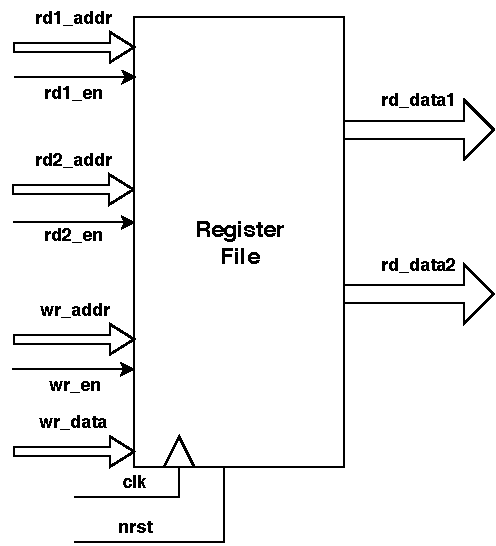
\includegraphics[width=.4\textwidth]{pics/RISCV_Core_RegFile.pdf}
	\caption{Register File Interface}
	\label{fig:regfile_interface}
\end{wrapfigure}

The Register File is a set of 32 registers, each one of 32 bits, with the only requirement that the \textit{X0} register is a read-only register that contains a $0$ value. It comes with two different implementations, one that consists of registers made of latches - if the target technology is ASIC - the other having registers made of flip flops - in case of FPGA. \newline
The interface of the module can be seen in the picture below:

For each input port there's the associated enable signal that controls the related operation: if wr\_en is $1'b1$, then it's possible to write the data presented at the wr\_data port at the address provided by the wr\_addr port (unless the address is equal to $5'h00$, in that case no writing operation is performed). The reading operation is performed in this way: for each port, if the related contorl signal is not enabled then the output will be equal to $32'h00000000$, otherwise the output will be the content of the register requested by rdx\_addr (x may be $1$ or $2$). If there's a read operation in parallel to a write operation and rs1==rd then the register will be written and the value at the wr\_data port will be forwarded to the output.

\section{Execute (EX1)}
In the Execute Unit the processor provides the correct operands (even in case of RAW hazard) to the ALU and evaluates the result of the operation required by the current instruction.\newline
This stage is comprised of the two aforementioned modules, the Forwarding Unit and the ALU, and two couples of multiplexers, two of them driven by the Forwarding Unit that selects the correct operand value based on the need to forward or not, the other two needed to select between \textit{op1\_execute} and \textit{pc} and between \textit{op2\_execute} and \textit{immediate\_field}. The output of the latter two MUXs will be the two inputs of the ALU.

\subsection{Forward Unit}
\label{fwdu}
\begin{wrapfigure}{R}{.55\textwidth}
\paragraph{}
\vspace*{-\parskip}	\centering
	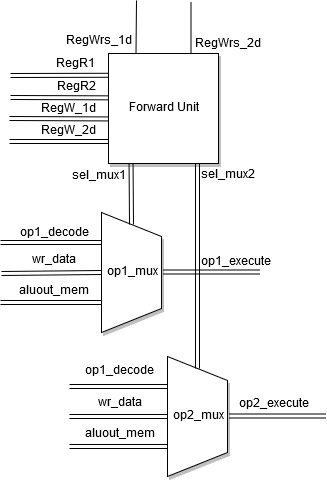
\includegraphics[width=.45\textwidth]{pics/ForwardUnit.png}
	\caption{Forward Unit}
	\label{fig:form}
\end{wrapfigure}
In a pipelined microprocessor, a Forward Unit (FWDU) is mandatory for preventing "bubbles" in the datapath pipeline in the event of a Read-After-Write (RAW) data hazard, that is the present instruction requiring the result of any of the previous two. 

To accomplish this task, the FWDU compares source registers of the current instruction with the other two's destinations, and if a collision is detected the appropriate forward path is enabled.

However, the present hazardous instruction may not intend to write a Register File (RF) location and instead simply use the address bits for another purpose, as is the case with load/store or immediate operations: to address this issue, the RF Write Enable signal is also fed to the FWDU.

The FWDU outputs two 2-bit buses, one per ALU input port, each controlling two muxes, each multiplexing between:

\begin{itemize}
    \item The RF output
    \item The ALU output
    \item The output of EX/MEM pipe register
\end{itemize}{}

This approach prevents any data hazard blocking the program execution, whereas with control hazards an additional module is integrated in the Control Unit, detailed in Chapter \ref{cu}.

\newpage

\subsection{ALU}
%list of operations
The unit is used to execute the 29 instructions we implemented that require arithmetic and/or logic operations. Depending on a control signal, named \textit{Control}, we can select the operation the ALU will perform; the organization is presented in the following table:
\begin{table}[h]
\centering
\begin{tabular}{@{}|cc|cc|cc|@{}}
\hline%\toprule
\textbf{Mnemonic} & \textbf{Coding} & \textbf{Mnemonic} & \textbf{Coding} & \textbf{Mnemonic} & \textbf{Coding} \\ \hline%\midrule
\multicolumn{1}{|c|}{LUI} & 4'b0000 & \multicolumn{1}{c|}{XORI} & \multirow{2}{*}{4'b0011} & \multicolumn{1}{c|}{SUB} & 4'b1001 \\ \cmidrule(r){1-2} \cmidrule(l){5-6} 
\multicolumn{1}{|c|}{LB} & \multirow{8}{*}{4'b0001} & \multicolumn{1}{c|}{XOR} &  & \multicolumn{1}{c|}{SLT} & \multirow{2}{*}{4'b1010} \\ \cmidrule(lr){3-4}
\multicolumn{1}{|c|}{LH} &  & \multicolumn{1}{c|}{ORI} & \multirow{2}{*}{4'b0100} & \multicolumn{1}{c|}{SLTI} &  \\ \cmidrule(l){5-6} 
\multicolumn{1}{|c|}{LW} &  & \multicolumn{1}{c|}{OR} &  & \multicolumn{1}{c|}{SLTU} & \multirow{2}{*}{4'b1011} \\ \cmidrule(lr){3-4}
\multicolumn{1}{|c|}{LBU} &  & \multicolumn{1}{c|}{ANDI} & \multirow{2}{*}{4'b0101} & \multicolumn{1}{c|}{SLTIU} &  \\ \cmidrule(l){5-6} 
\multicolumn{1}{|c|}{LHU} &  & \multicolumn{1}{c|}{AND} &  &  &  \\ \cmidrule(lr){3-4}
\multicolumn{1}{|c|}{SB} &  & \multicolumn{1}{c|}{SLLI} & \multirow{2}{*}{4'b0110} &  &  \\
\multicolumn{1}{|c|}{SH} &  & \multicolumn{1}{c|}{SLL} &  &  &  \\ \cmidrule(lr){3-4}
\multicolumn{1}{|c|}{SW} &  & \multicolumn{1}{c|}{SRLI} & \multirow{2}{*}{4'b0111} &  &  \\ \cmidrule(r){1-2}
\multicolumn{1}{|c|}{ADDI} & \multirow{3}{*}{4'b0010} & \multicolumn{1}{c|}{SRL} &  &  &  \\ \cmidrule(lr){3-4}
\multicolumn{1}{|c|}{ADD} &  & \multicolumn{1}{c|}{SRAI} & \multirow{2}{*}{4'b1000} &  &  \\
\multicolumn{1}{|c|}{AUIPC} &  & \multicolumn{1}{c|}{SRA} &  &  &  \\ \hline%\bottomrule
\end{tabular}
\end{table}
\section{Multiplication and Division Unit (EX2)}
%Digital arithmetic is nowadays well known and implemented in various applications and products. After technology scaling has become slower, the need of more advance technology in terms of performances, energy consumption and occupied area brought more focus on the development of better architectures. The strength of the major companies in the area of general purpose microprocessors stands also here.\\
The present unit implements multiplication and division operations and takes a less academic approach to the matter. While almost all algorithms are well described in literature, the implementation still is left to hardware designers, which brings issues about especially having different data formats in the same architecture.
\subsection{Specifications}
The unit must execute correctly all the RV32-M instructions, so each operation must be capable to handle both signed and unsigned numbers, or even mixed types.

Official RISC-V Foundation specifications also explicitly ask that in case of :
\begin{itemize}
    \item Consecutive \textit{MULTH[S][U]} and \textit{MULT} 
    \item Consecutive \textit{DIV[U]} and \textit{REM[U]}
\end{itemize}
Where \textit{rs1} and \textit{rs2} sections are equal, the unit must immediately provide the correct result without performing again the same computation.
Lastly \textit{division by zero} and \textit{division overflow} must rise two different exceptions. It's important to notice that the first case is the only arithmetic trap in the standard ISA, for which we are not providing any interaction with the execution environment’s trap handlers. Anyway division by zero must cause an immediate control flow change and only a single branch instruction can be inserted before every division one, which will be very predictably not taken.
METTERE LA FOTO DEI CASI SPECIALI DIVISIONE
\newpage
\begin{figure}[H]
    \centering
    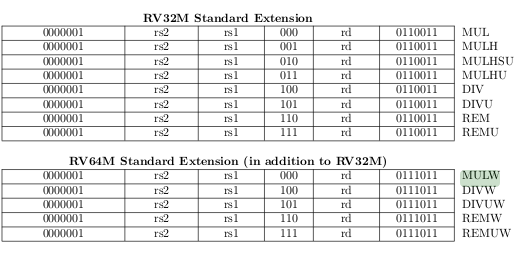
\includegraphics[scale=0.7]{pics/complete.png}
    \caption{RV32M and RV64M instructions}
    \label{fig:my_label}
\end{figure}
\subsubsection{Algorithms chosen}
After a first research on how modern microprocessors perform multiplications and divisions, the most common solution was found to be a shared microprogrammed architecture based on sequential algorithms: \textit{Booth encoded multiplication} and \textit{Sweeney-Robertson-Tocher division}. A short description of both can be found on the following sections.\\
This is mainly for three motivations:
\begin{itemize}
    \item Both algorithm can share the same basic hardware blocks. 
    \item Working on sequential architectures opens to several possible improvements on the critical path, avoiding any frequency issue inside machines that tends to achieve shorter and shorter periods. Also low-power techniques can be easily implemented during design time. Since both operations share the same architecture any upgrade done for one may be applicable also for the other.
    \item Algorithms can be modified to elaborate more steps in a single clock cycle with very low timing overhead. Those algorithms are addressed as \textit{higher radix}.
\end{itemize}
The proposed implementation focuses just on the first two points, while was chosen to keep the simple radix-2 algorithms because higher ones would lead to longer design time. But once an eventual high-radix algorithm is set up for the specific case, few modifications on the radix-2 architecture may be needed.
\subsubsection{The use of carry save adder}
The kernel of the recipes for multiplication and division is made of additions and shifts repeated for a certain amount of cycles. The first improvement suggested by sources on computer arithmetic was to use a carry save adder and store the result of each iteration in the sum-carry form.\\
Partial reminder and partial product will be taken as just said. Then final result has to be computed by a "normal" sum, for which any kind of adder can be used, except for the one used in the kernel cycles.\\
While for the multiplication introducing this amendment is not a big deal, for division brings some issues, since the operations that must be performed in each step of it depends on the value of the partial reminder at the previous one. The point is that there is no way to know it, when it is expressed in the sum-carry form, without performing a sum of the two parts. This would cancel all the efforts.\\ 
What can be done is to guess the partial reminder looking just at the first 5 bits of sum and carry and then implement some mechanism that corrects the result in case of one or more mistakes done during the elaboration.\\ In few words, performing some approximate computations the divisor architecture is capable to produce at the end an exact result.
\subsection{Multiplication}
Multiplication can be considered much easier to handle then division. As previously said, the carry save adder choice doesn't affect much the design.\\
\subsubsection{Theory explanation}
Architecture is based on the \textit{right shift} algorithm, in which for each step a partial product is computed by multiplying the multiplicand by a bit of the multiplier starting from the rightmost one, then it is summed to a partial result obtain from all the previous steps and finally, the number got, is divided by 2:
\begin{equation}
    p^{(j+1)}=(p^{(j)}+2^k*x_ja)2^{-1}
\end{equation}
Where:
\begin{itemize}
    \item \textit{$p^{(j)}$} is the partial result at the generic step \textit{j}.
    \item \textit{$x_j$} is the bit of the multiplier at \textit{j} position starting counting from the lsb.
    \item \textit{k} is the number of bits. In this case 32.
    \item \textit{a} is the multiplicand.
    \item \textit{$p^{(0)}$} is equal to \textbf{0}.
    \item \textit{$p^{(k)}$} is the product of the multiplication.
\end{itemize}
\paragraph{Booth encoding}
Partial products' value may be equal to \textbf{a} if the corresponding multiplier bit is equal to 1 or \textbf{0} in the other case. Performing a multiplication where most control bit are zeros requires less effort than in the opposite possibility. Booth exploited this simple tip re coding multiplier's bit. This operation consists in replacing a sequence of 1s, all additions, with a subtraction at the least-significant end an addition in the position immediately to the left of its most-significant end. As an example
\begin{center}
    \textit{011110} will become \textit{1000-10}
\end{center}
It's possible to obtain from \textit{$x_j$} bit a new \textit{$y_j$} re coded one as follows:
\begin{table}[H]
    \centering
    \begin{tabular}{c|c|c|c}
        $x_j$   & $x_{j-1}$ & $y_j$ & Explanation   \\
        \hline
        0       &   0        &  0     & No string\\   
        0        &      1     &  1      & End of string              \\
        1        &       0    &   -1    &       Beginning of string  \\
        1        &       1    & 0      &  Continuation of string             \\
    \end{tabular}
    \caption{Booth re coding table}
    \label{tab:my_label}
\end{table}
With this re coding we obtain another important feature: now the multiplier can also handle signed operands, while normal right shift one couldn't. In this way is also possible to satisfy 

\subsubsection{Model}
The algorithm for the Booth re coded multiplication can be modeled with the following python code
\begin{minted}[fontsize=\footnotesize]{python}
BE_multiplier (multiplicand,multiplier,signed_unsigned_n,parallelism):
    #converting multiplier in it's equivalent string of bits
    mult_string=printer_2s(multiplier,parallelism)
    a=multiplicand*(2**(parallelism-1)) #a*2^k
    #first case in which there is not x(j-1)
    if (int(mult_string[parallelism-1])): #checking LSB
        p=-a
    else:
        p=0
    p=p/2
    for i in range(0,parallelism-1):
        if mult_string[parallelism-i-2]=='0' and mult_string[parallelism-i-1]=='0':
            p=p
        elif mult_string[parallelism-i-2]=='0' and mult_string[parallelism-i-1]=='1':
            p=p+a
        elif mult_string[parallelism-i-2]=='1' and mult_string[parallelism-i-1]=='0':
            p=p-a
        else:
            p=p
        p=p/2
    p=p*2
    return p
\end{minted}
\subsubsection{DataPath}
For the realization of the multiplier's datapath only simple basic blocks are needed. 
\paragraph{Kernel Logic}
The logic for the selection of the generic partial product is very simple. Two signals are needed:
\begin{itemize}
    \item NonZero: obtained with an XOR gate between $x_j$ and $x_{j-1}$
    \item Negative: obtained with a direct connection with $x_j$
\end{itemize}
It's important to notice that first partial product is directly loaded with the multiplier and it's chosen using its least significant bit.
\paragraph{Final adder}
The final adder is not implemented. Synthesizer will choose a model of adder and place it after synthesis. This will remain true also for the divisor.
\paragraph{Counter}
For reasons of space the counter is omitted in the schematic. A signed multiplication would require only 32 steps, while an unsigned one takes always 33 steps because the case in which $32^{nd}$ bit, most significant bit, is 1 must be taken in account and a 0 must be put at the left end of the number to correctly handle the operation.\\
In order to simplify control and the finite state machine, the machine always performs 33 steps which will always give the right result. A clock cycle is lost for every signed multiplication.\\
Considering that the first step is automatically done while loading the multiplier in the \textit{sumH} register, the counter must count only 32 multiplication steps. Latency is always the same.\\
\begin{figure}[H]
    \centering
    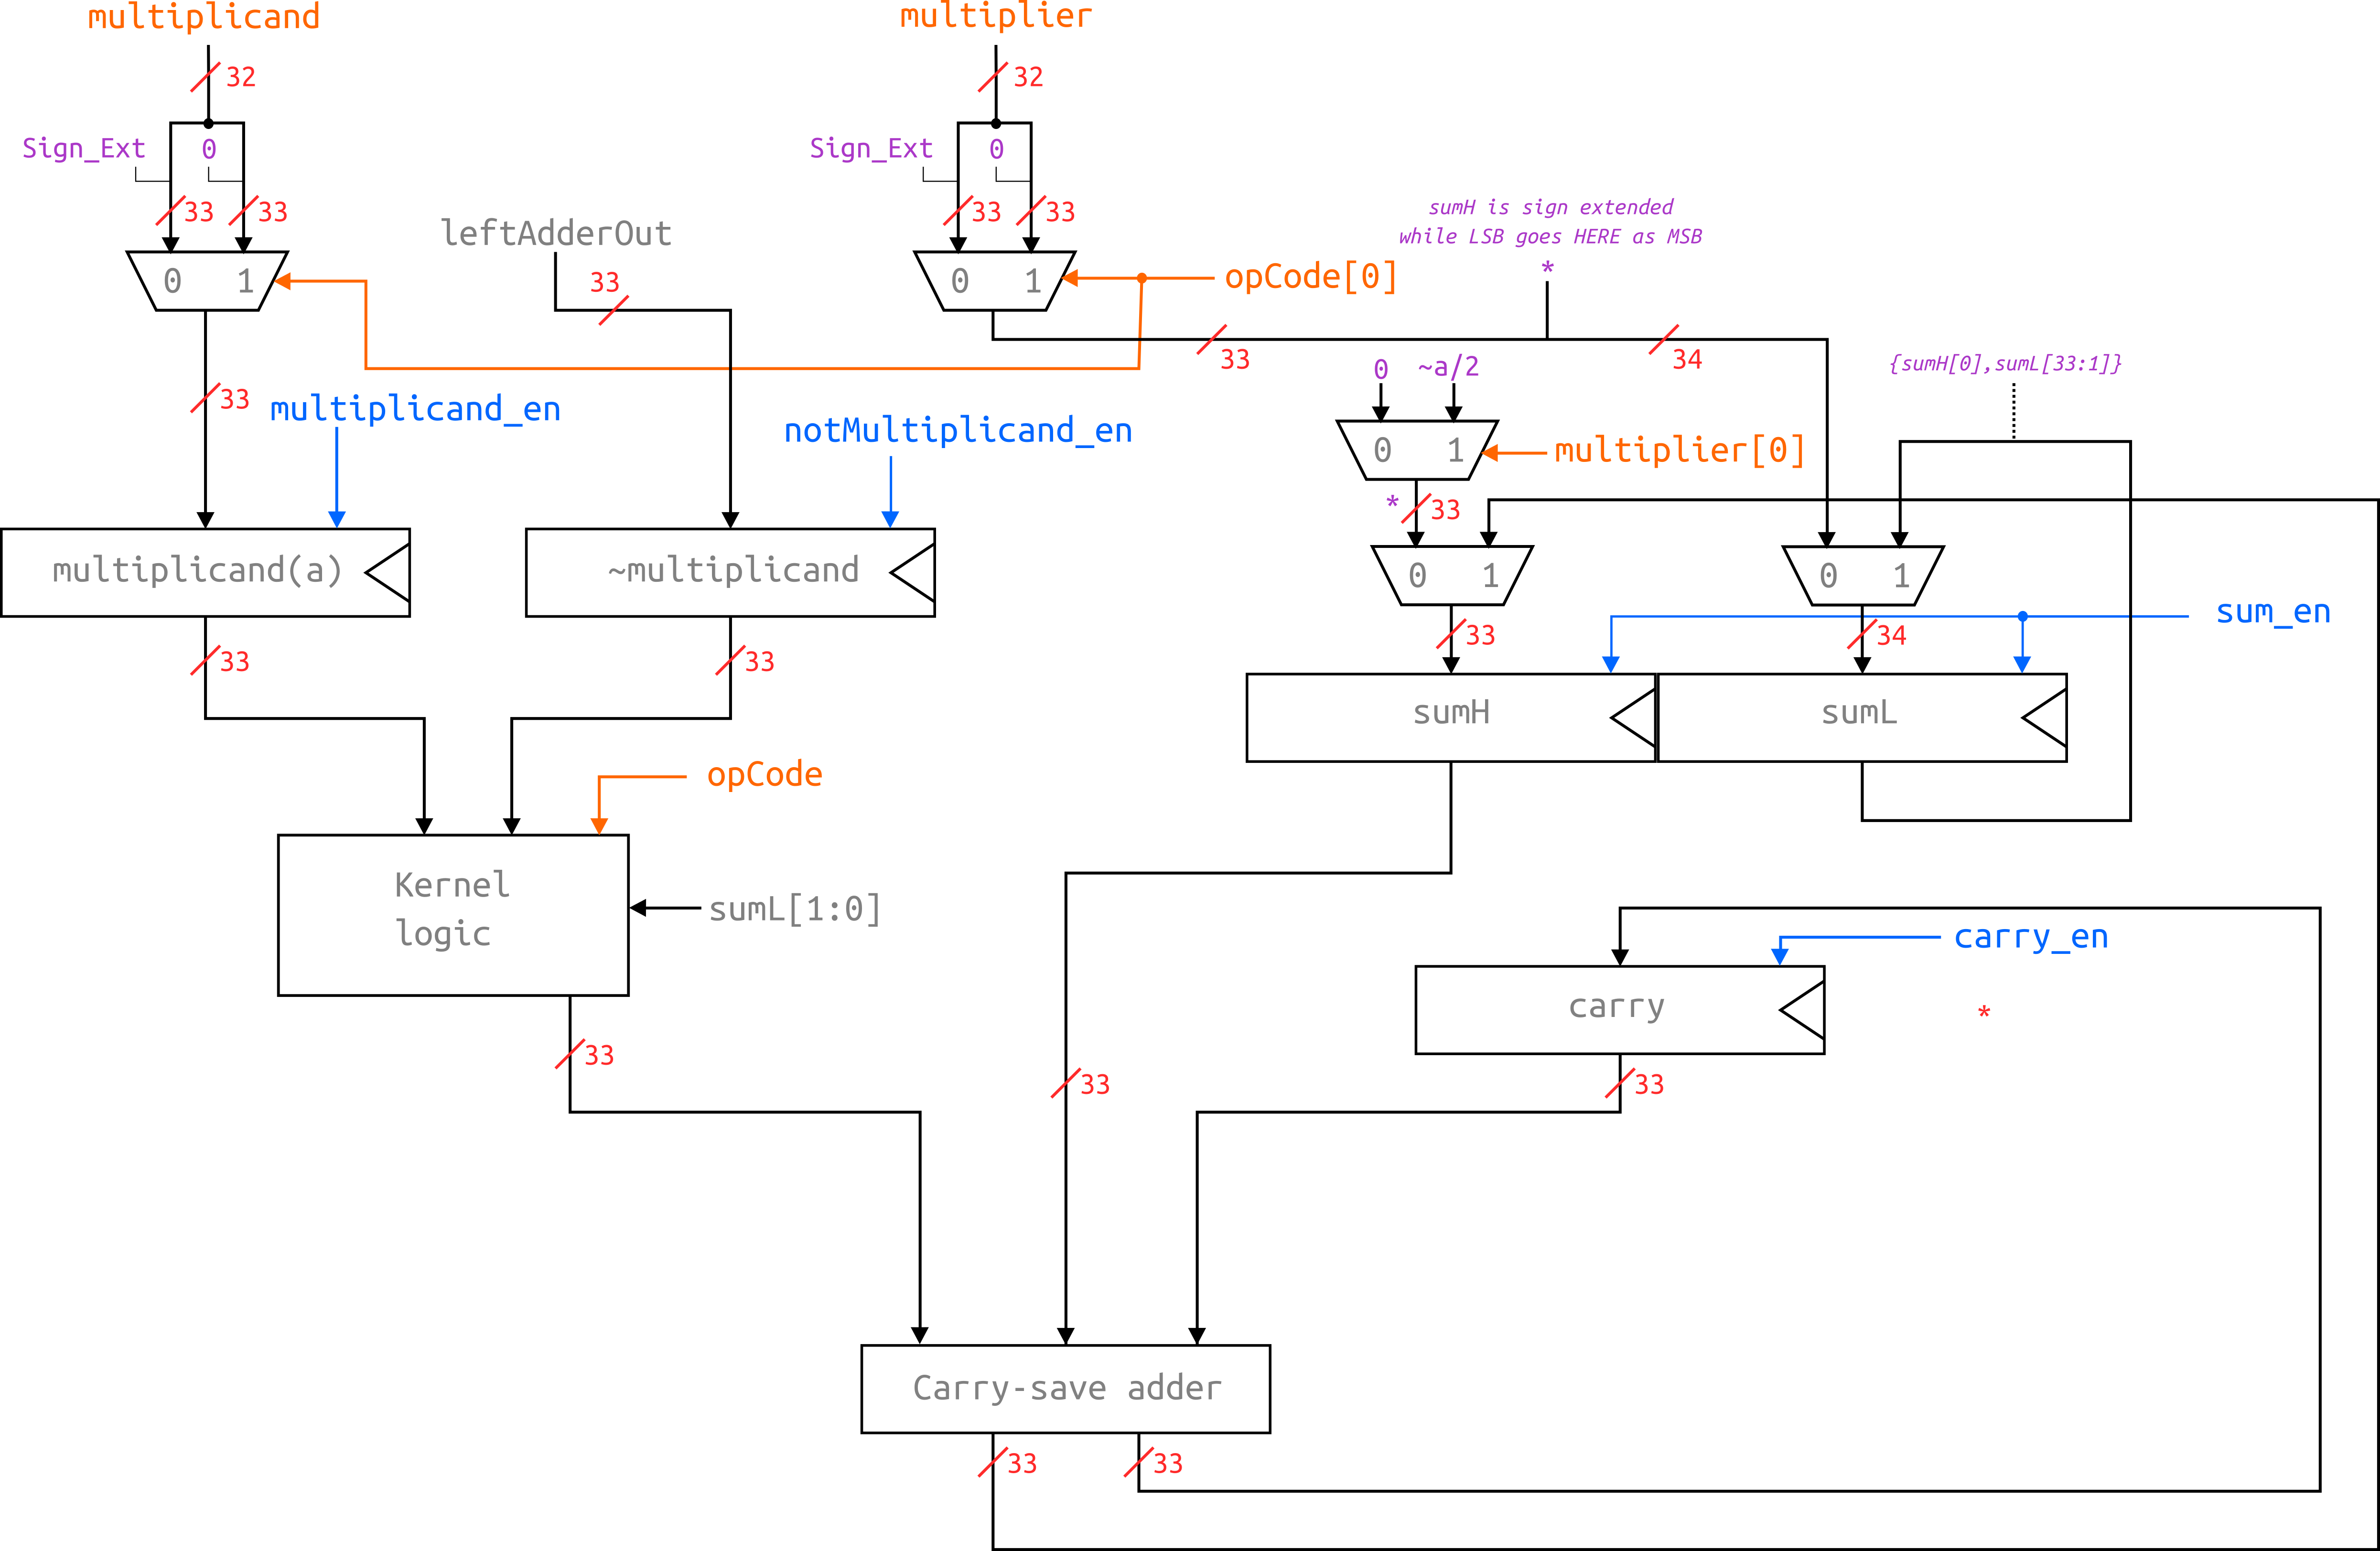
\includegraphics[angle=90,scale=1]{pics/multiplierKernelCircuit.png}
    \caption{Multiplier upper datapath}
    \label{fig:my_label}
\end{figure}
\begin{figure}[H]
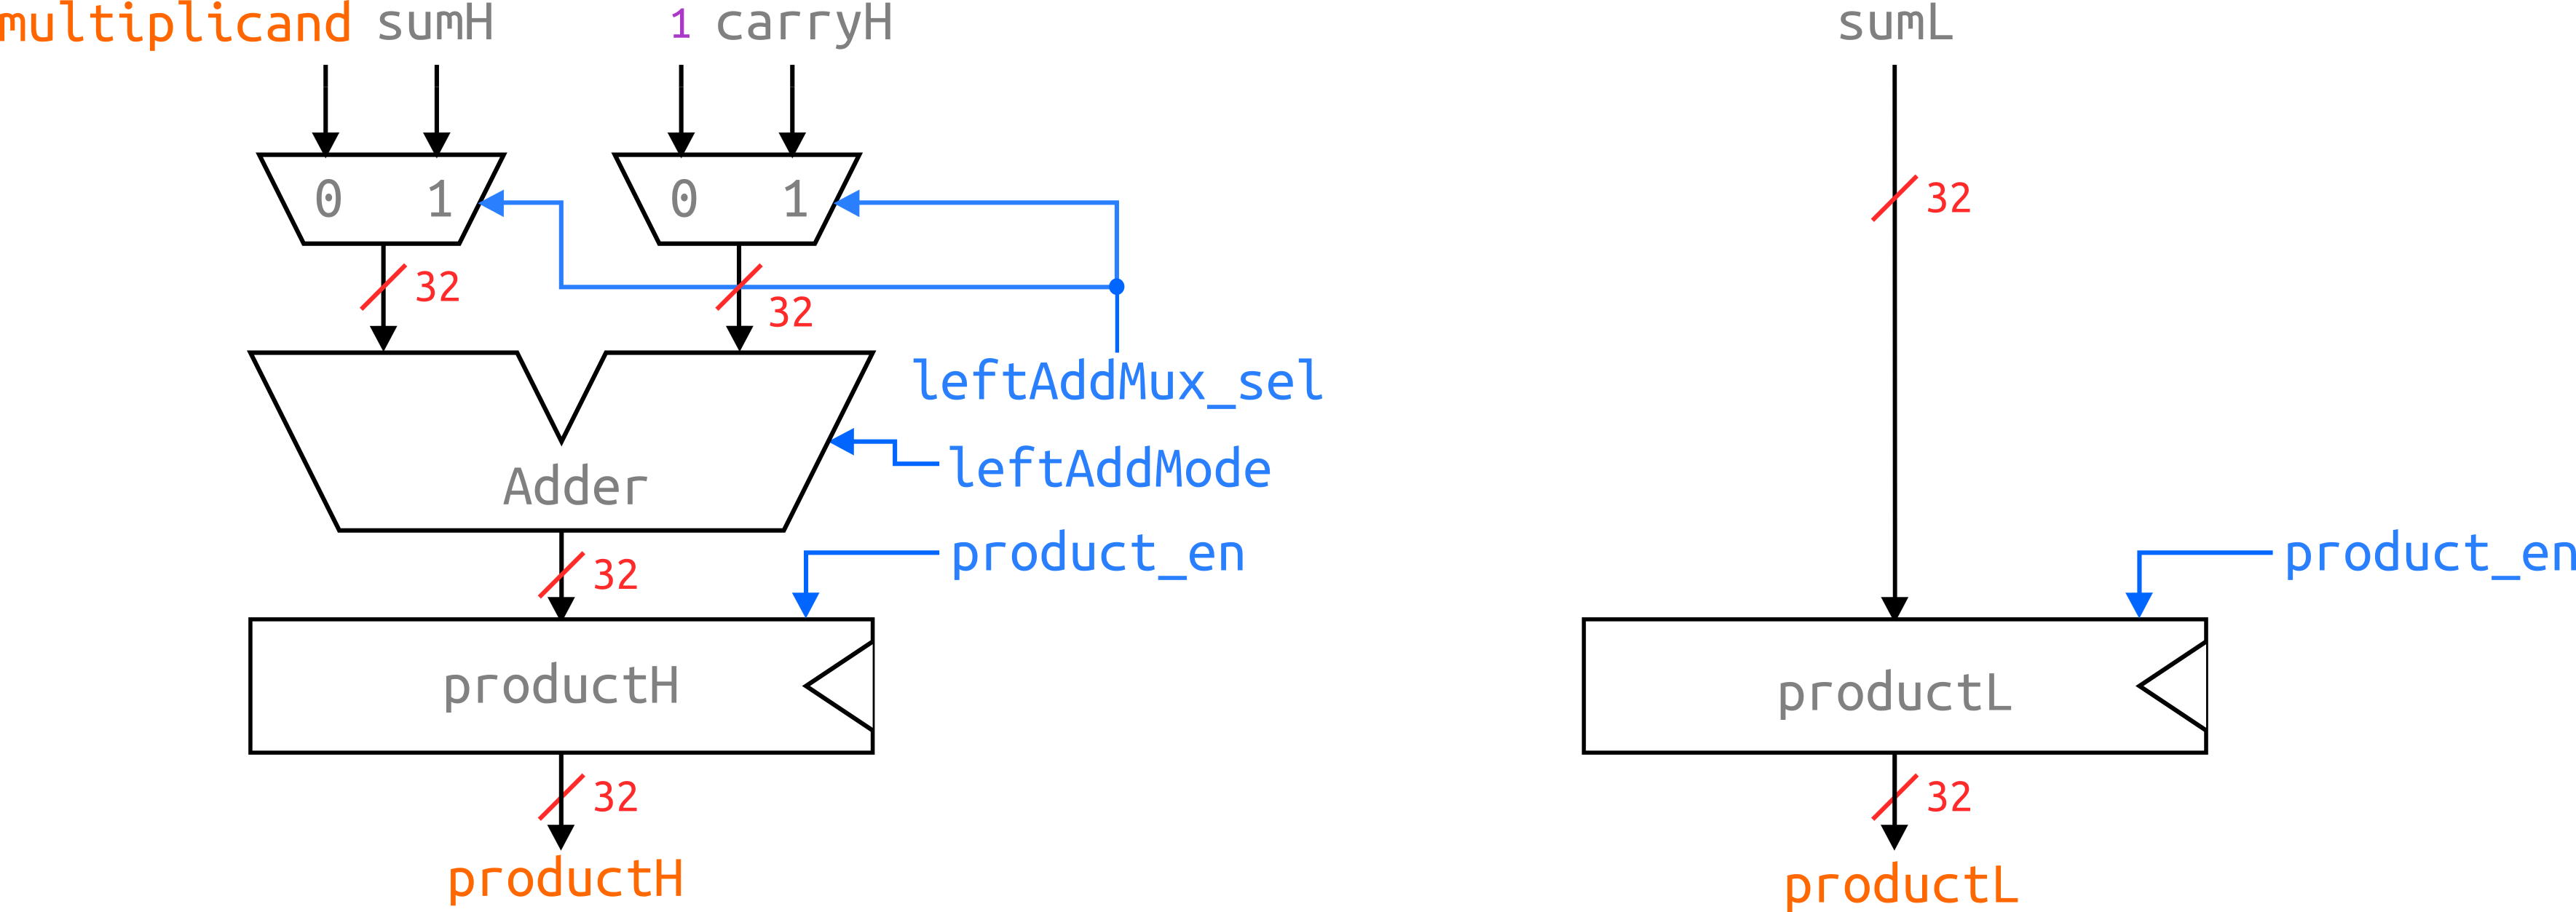
\includegraphics[scale=1]{pics/multiplierOutReg.png}
    \caption{Multiplier lower datapath}
    \label{fig:my_label}
\end{figure}
\subsubsection{Finite state machine}
Few controls for the whole multiplication are needed.
\paragraph{\textit{idle} State}
The machine waits in the idle state until a specific signal is raised by the outer world, communicating that operands are valid and need to be evaluated. The only operation performed is a synchronous clear of the sum and carry registers. This is because an asynchronous reset signal controlled by a finite state machine may lead to problems in the post synthesis circuit, since spurious glitches in the output logic of the commands may reset the entire circuit when unwanted.
\paragraph{\textit{save\_multiplicand} State}
Only the multiplicand register is enable, before its negative value must be computed before loading the multiplier.
\paragraph{\textit{save\_multiplier} State}
The multiplexers at the input of the adder in the lower part of the data path must be set correctly in order to compute the \textit{negative multiplicand ($-a$)}. Least significant bit of multiplier will select the correct partial product, that will be loaded with the multiplier in the \textit{sum} registers.
Computing $\textit{-a}$ isn't essential for the purposes of the algorithm. In fact it's possible to add the bit-wise not of the multiplicand to the partial result when required, and store the +1 bit for making the 2's complement in another register. Then at the end, all these +1 bits, in the appropriate weight, can be summed together to the final result, saving one state in the finite state machine.\\
Since for the division is mandatory to compute the negative value of the divisor, the same is done for the multiplication, simplifying a bit the design.\\
\begin{figure}[H]
    \centering
    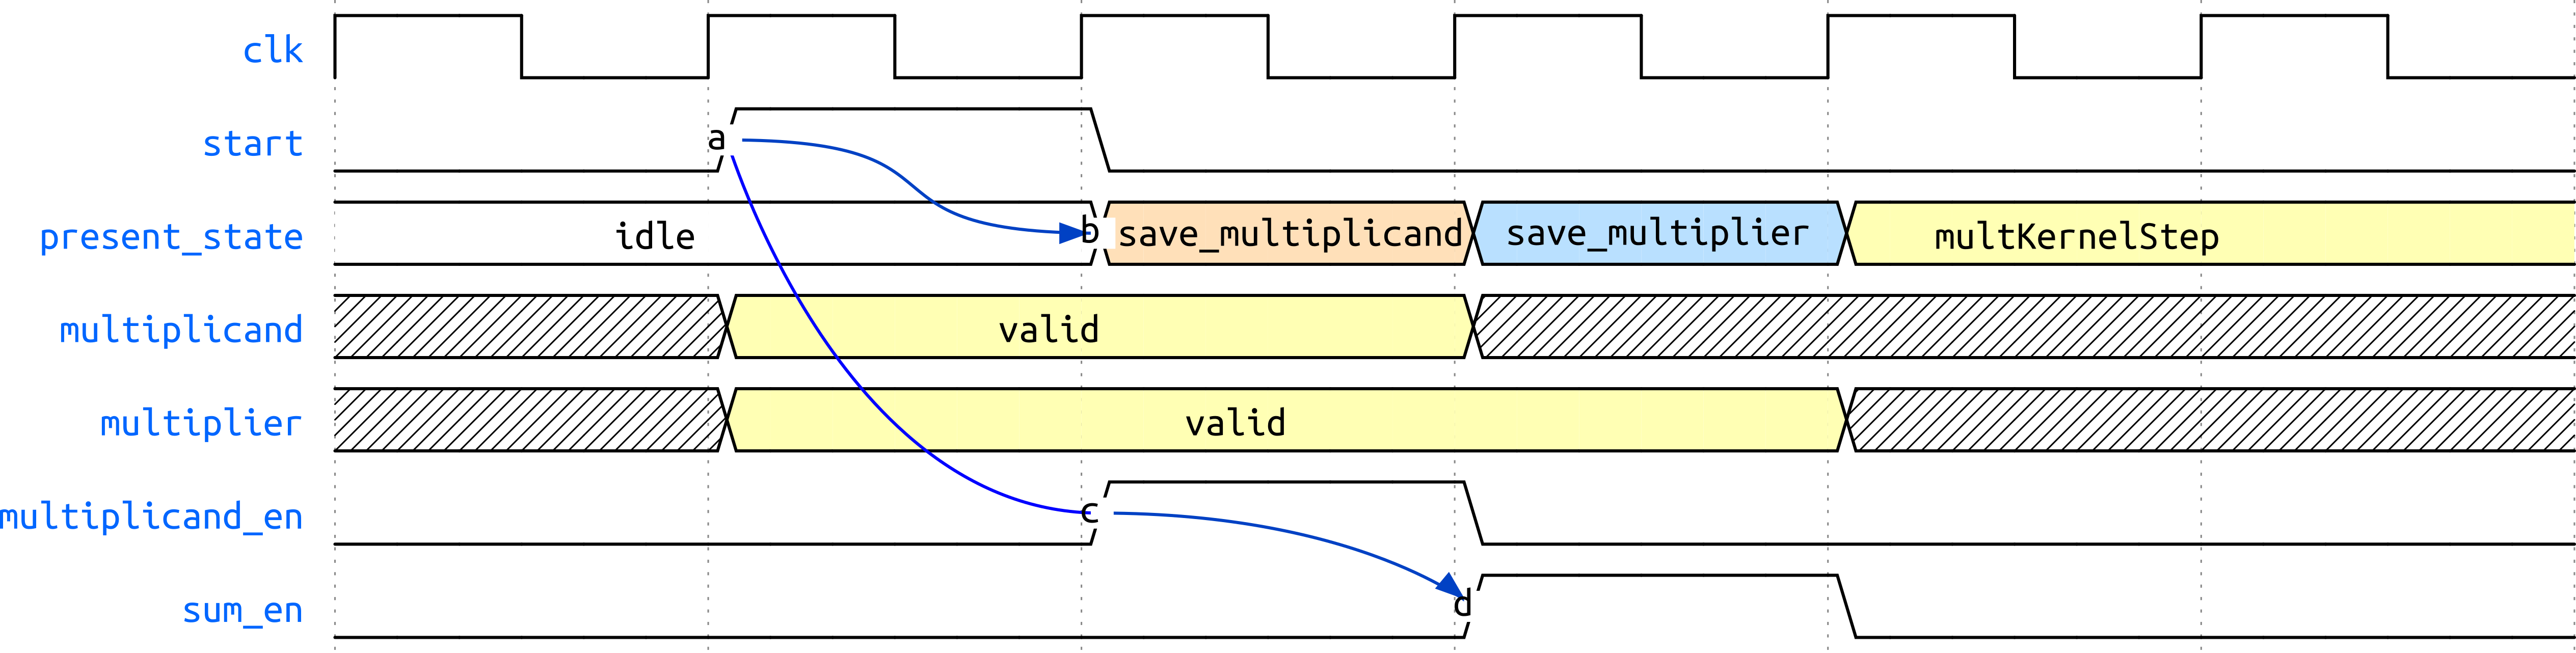
\includegraphics[scale=0.7]{pics/multStart_wave.png}
    \caption{Timing of the starting operation}
    \label{fig:my_label}
\end{figure}
Notice that multiplier must remain valid for at least \textbf{three clock cycles} after the rising edge of the \textit{start signal}.
\paragraph{\textit{multKernelStep} State}
After first step is performed, 32 always equal are left. For each one of these the correct partial product must be selected and added to the partial result as explained before. The division by 2 is automatically done storing the output of the carry save adder shifted to the right, the least significant bit of the \textit{sum} goes in the most significant one of the register that initially was holding the multiplier, which is also shifted in order to update control bits for the choice of the next partial product.
%magari schema ingresso registri somma
\paragraph{\textit{save\_product} State}
Final product will be made up by two words of 32 bits. The most significant one is expressed in the sum-carry form and must be computed by summing the two parts, while the least significant is already ready and stored in the \textit{sumL} register in the range that goes from $33^{rd}$ to the $2^{nd}$ bit.
%magari schema ingresso adder di uscita
\paragraph{\textit{multDone} State}
End of computation is signaled to the outer world.
\begin{figure}[H]
    \centering
    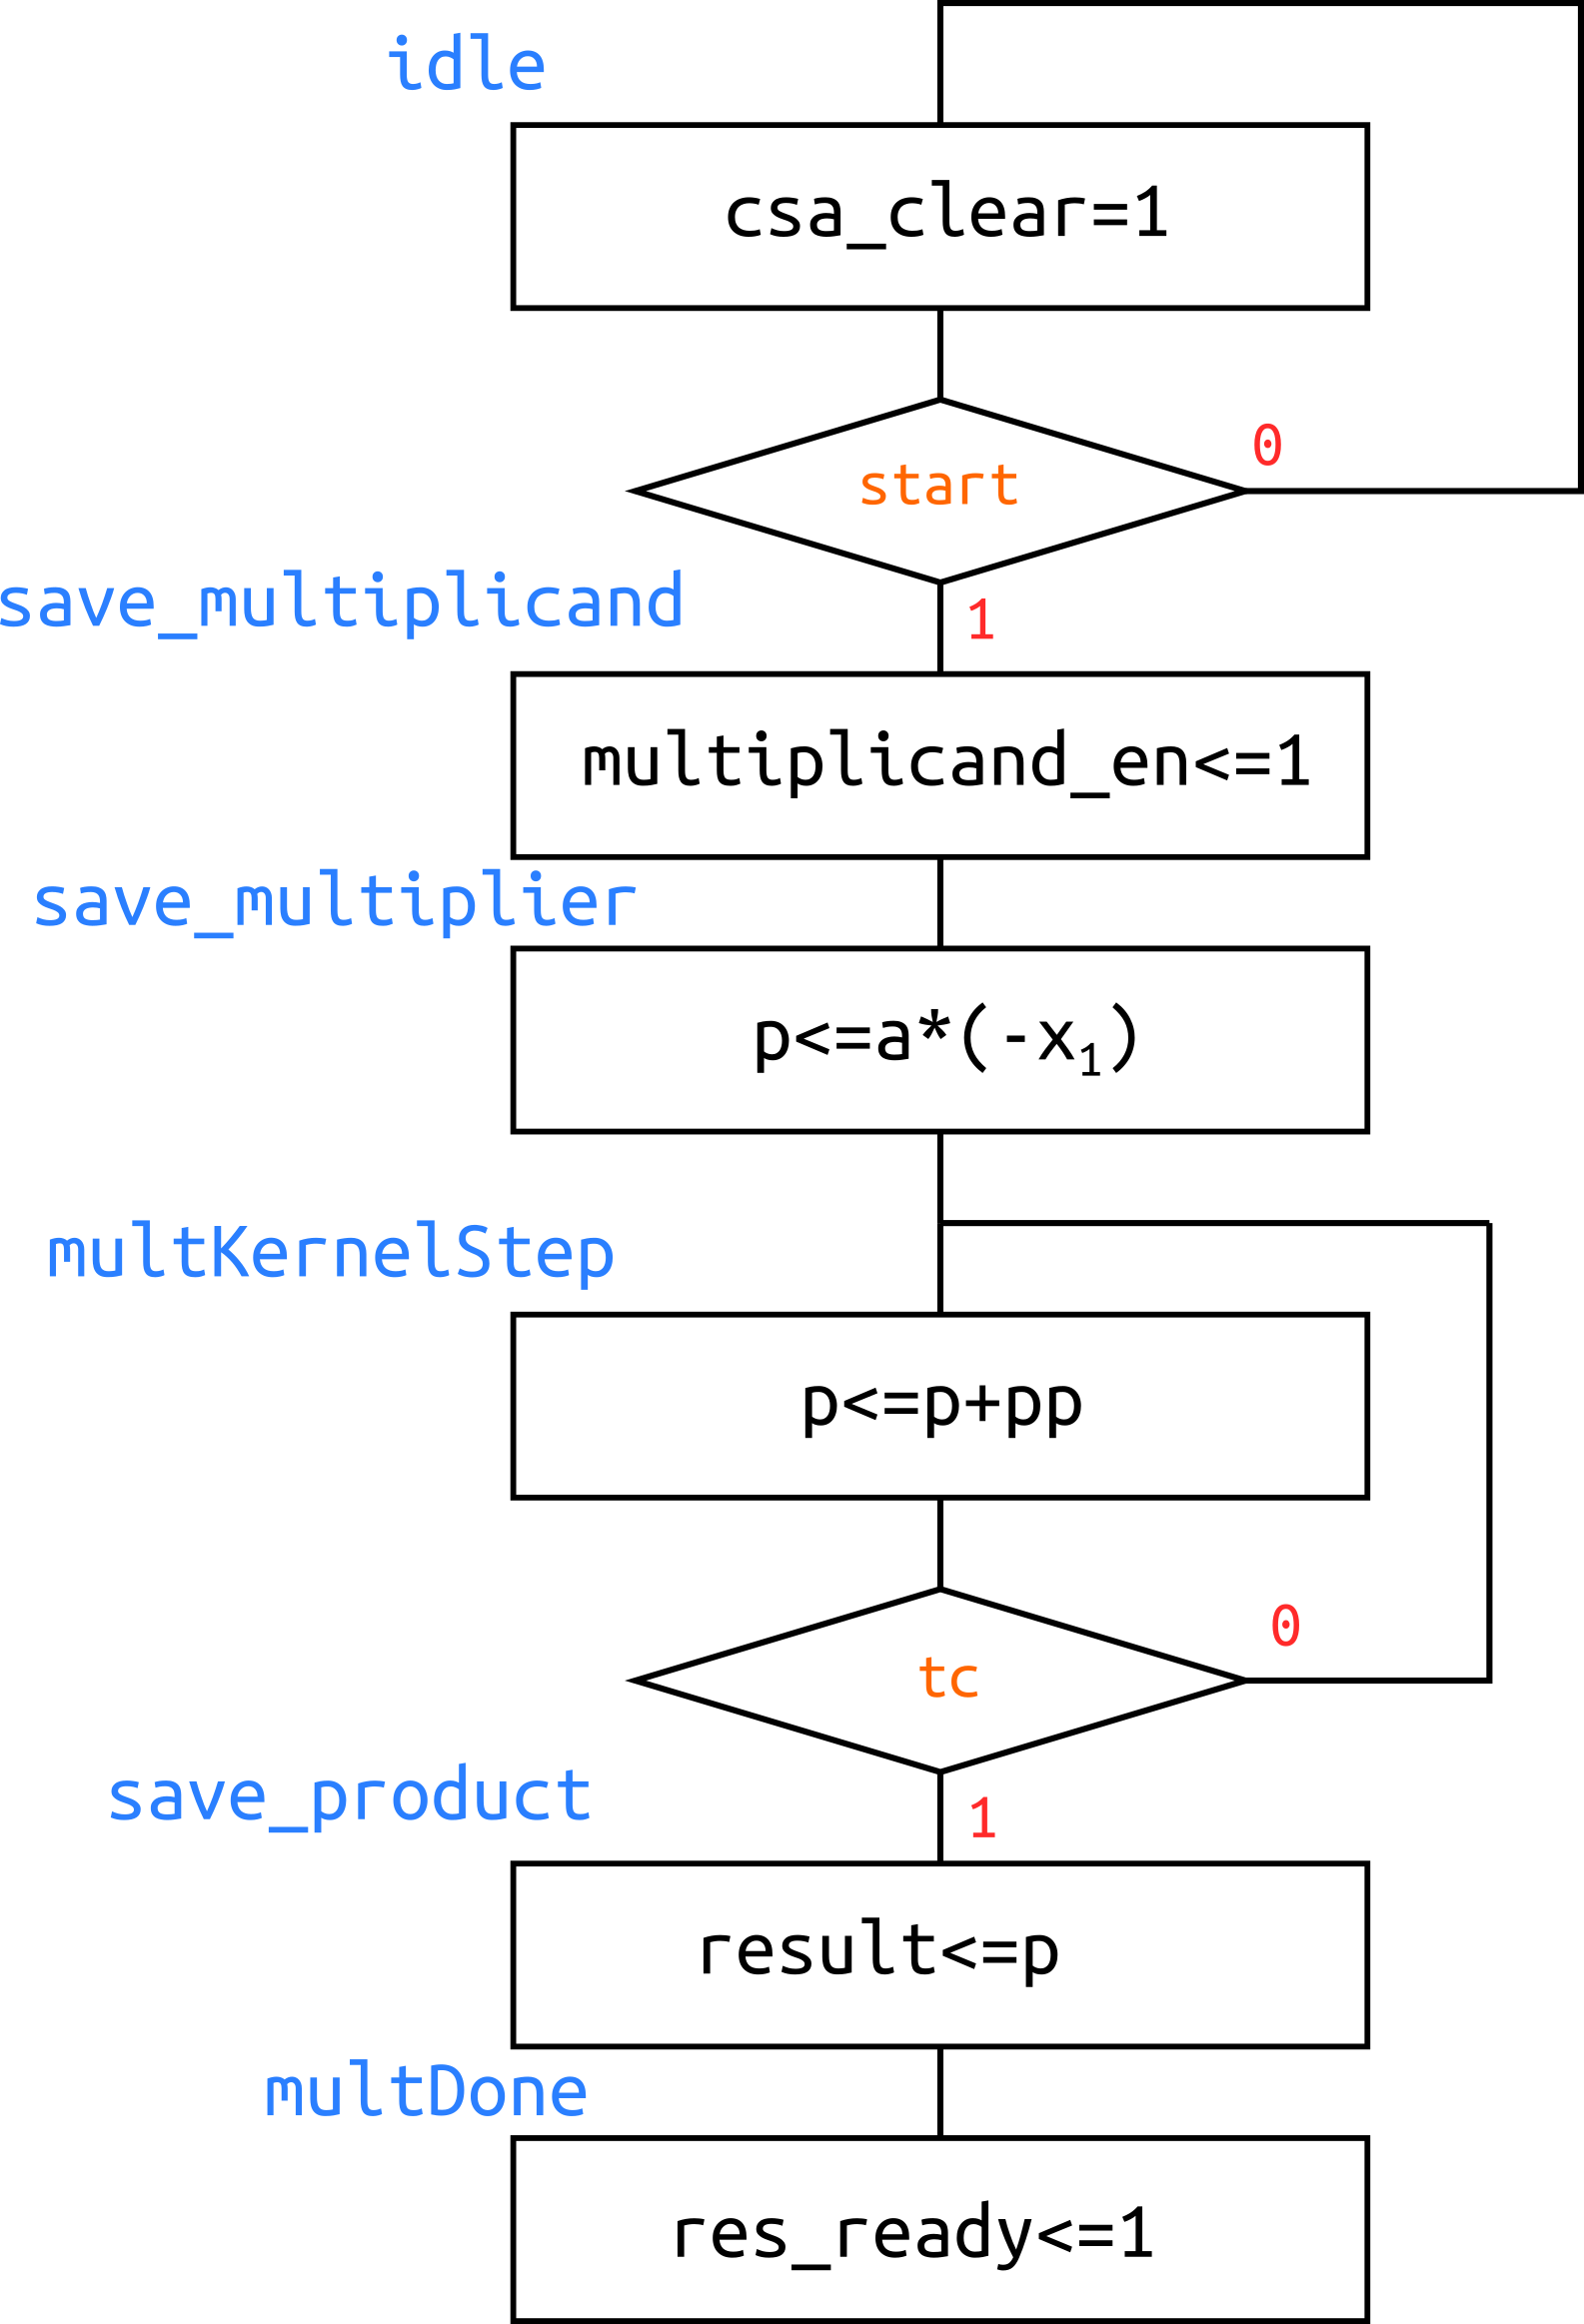
\includegraphics[scale=1]{pics/multiplierASM.png}
    \caption{Multiplier ASM}
    \label{fig:my_label}
\end{figure}
\begin{figure}[H]
\centering
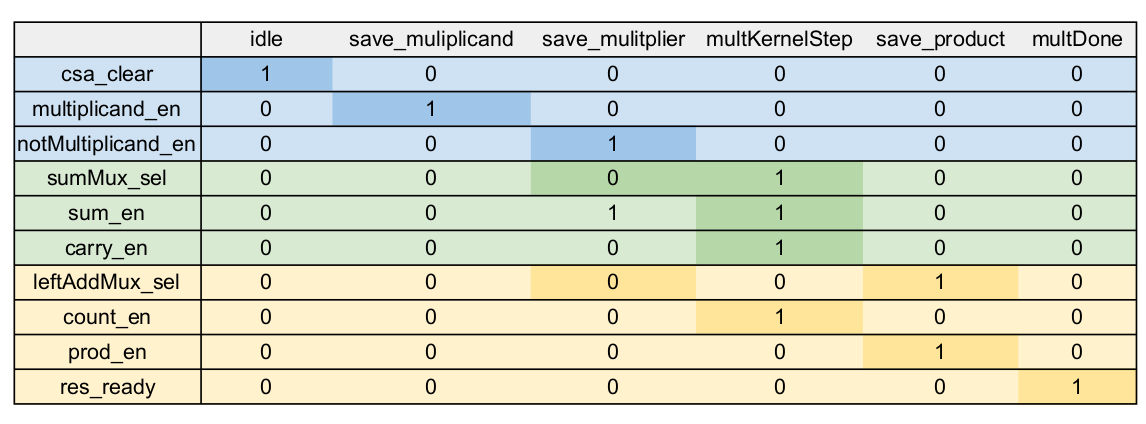
\includegraphics[scale=0.35]{pics/multControl.png}
    \caption{Multiplier control signals}
    \label{fig:my_label}
\end{figure}

\subsection{Division}
Very complex and tricky was the design of the divisor. There are three main motivations that contributed to make intricate the realization of a division machine:
\begin{itemize}
    \item available algorithms are not general. Re conducing all possible cases to the specific ones described in literature it's not trivial. What has to be realized is a machine that can handle two operands, signed or unsigned, of 32 bits, but with unknown actual dynamic (e.g. how many bits are sign extension). SRT division is described only for dividend of twice the number of bits respect to the divisor, which must also respect some strict conditions. 
    \item Design, at the beginning, is base on some considerations that may be wrong, but can't be verified at priory. Those assumptions introduce some bug inside a partially working machine that are hard to detect or understand. The only way is to analyze bit by bit the internal behavior, which is a very stress full job, error prone and takes most of the design time.
    \item all number are expressed in fixed point format, but due to different type of operations done in the division kernel, the number of bits assigned for the integer and the fraction may vary across the architecture in order to avoid overflows and unused resources. For example 2.30 format can be extended to 3.30 which is totally different from 2.31, even if they are bot 33 bits data. Or also 2.30 can be truncated to 2.29 if lsb is not needed, but must be handled assigning the right weight to every bit.
    \item some tasks in the algorithm can be \textit{"commutative"}, the order doesn't count for the final result, but can make the design much more complex. 
\end{itemize}
\subsubsection{Theory explanation}
Explaining all the theory that lays under the division algorithm is long and complex, this will be a very short recap. For more information please consult the bibliography.\\
\paragraph{Basic algorithm}
The starting point for the model of the final divisor is the \textit{non restoring and signed division}.\\ 
The main procedure lays on the these hypothesis:
\begin{itemize}
    \item Dividend can be expressed in \textit{2k} bits while the divisor in half of the width, just \textit{k} bits.
    \item The value obtained by multiplying the divisor by $2^k$ must be strictly less than the dividend. If this condition isn't true an overflow can verify at the first step of the algorithm.
\end{itemize}
 We can generally say that
 \begin{equation}
     z=qd+s
 \end{equation}
 Where \textbf{z} is the dividend, \textbf{q} is the quotient, \textbf{d} is the divisor and \textbf{s} is the reminder.\\
 The operation done in one of the basic steps \textit{j} out of 32 can be then expressed as
 \begin{equation}
     s^{(j)}=2s^{(j-1)}-q_{k-j}*2^kd
 \end{equation}
which is the same as for the restoring algorithm. What changes is that in case the subtraction performed leads to a sign change in the partial reminder, no restore and change of the value of the quotient bit is performed, but in the following step an addition is applied.
The effect of this trick can be easily demonstrate.
\begin{equation}
     s^{(j+1)}=2s^{(j)}+2^kd
 \end{equation}
 Substitution of $s^{(j)}$ leads to:
 \begin{equation}
     s^{(j+1)}=4s^{(j-1)}-2*2^kd+2^kd
 \end{equation}
 The only thing that must be done is to keep track of what operation has been performed for each step in the quotient.\\
 If $sign(s^j)=sign(d)$, $q_{k-j}$ is set to \textit{1}. In the opposite case it is set to \textit{-1}. \\
 At the end, it's possible to obtain two numbers, the one made of \textit{1} and the other made of \textit{-1}. To get the quotient is enough subtracting the twos.\\
 Before producing the result is mandatory to check if the reminder is coherent with the dividend, if it's not a correction step must be provided to recover the mistake. If sign($s^k$)=sign(d) it means that d must be subtracted to $s^k$ and quotient incremented, if it's not 
an addition is needed and quotient is decremented.\\
\paragraph{SRT division}
The \textit{Sweeney-Robertson-Tocher division} is based on the idea that it's possible to avoid any addition or subtraction in a normal kernel step if the partial reminder is enough "small". If it is in the range $[-d,d)$, multiplying it by two, it's possible to choose $q_{k-j}$ equal to 0.\\
%%mettere le immagini delle soglie, prese dal libro
The problem of this concept is that is not possible to compare the partial reminder with the divisor without subtracting them and then analyze the result with extra logic. This would slow down dramatically the architecture.\\ The only way to undo the knot is to choose easy fixed thresholds for the comparison, it's possible to achieve this by expressing the operands in fixed point 1.31. Then two conditions must hold:
\begin{itemize}
    \item $d \geq 0.5$, if it's not true divisor must be shifted left. The number of shifts will become the number of kernel step that must be performed. It's important to remember that the reminder must be corrected at the end by shifting it right the same amount of time.
    \item $-d \leq z < d$, if it's not true dividend must be shifted right once, then result must also be realigned at the end. In the design z is always divided by 2, so that this condition is always true.
\end{itemize}
Two comparison are still needed to select the correct quotient digit, but now they can be done with two constants: $-0.5$ and $0.5$. This implies just a logic gate layer.\\
%mettere immagini degli intervalli
\paragraph{Carry Save adder}
Carry save adder, as for the multiplication, speeds up the computation done each cycle.\\
But imagine if partial reminders must be stored in the sum-carry form. The only way to determine it's actual is to compute it. This would null all the advantages obtained introducing the carry save adder. What can be done is to sum just the most significant bits up to second decimal place and modify thresholds to handle the case in which the actual number falls outside the range with an approximate computation. The sum can be implemented with a look-up table or a PLA in order to in crease the access speed.\\
In literature, it's written that only two guard bits are needed to avoid overflows after the sum, but what was found during the design is that there are cases, one over two thousand, in which one more is needed for the carry register. So in the schematic 5 bits are used for the quotient bit selection.
%immagine nuove soglie e p-d plot

\subsubsection{Model}
All the steps described in the previous part are resumed in the following python code, which is as close as possible to what the hardware machine really do.
\begin{minted}[fontsize=\footnotesize]{python}
#thr1=0 and thr2=-0.5 in this case
def SRTr2_divisor(dividend,divisor,inPar,thr1,thr2):
    #division by zero case
    if (divisor==0):
        return "divisorIs0"
    #fixed point format 1.33
    #division inPar+1 for both signed and unsigned case, -d<=z<d always true
    z=dividend/2**(inPar+1)
    d=divisor/2**(inPar+1)
    #first step s(0)=2*z
    s=z*2
    #shifting left divisor until more than 0.5
    loop_iteration=0
    while ((d<0.5 and d>0) or (d>=-0.5 and d<0)):
        loop_iteration+=1
        d=d*2
    #standard kernel iterations
    q=""
    for i in range(0,loop_iteration):
        if(s>=thr2):
            _q=1
            if (d>0):
                s=s-d
            else:
                s=s+d
        else:
            if (s>=thr1):
                _q=0
                s=s
            else :
                _q=2
                if (d>0):
                    s=s+d
                else:
                    s=s-d
        s=s*2
        q=q+str(_q)
    #last step doesn't require *2, so a correction is needed
    s=s/2
    #quotient conversion
    quotient=0
    for i in range(0,loop_iteration):
        if (q[len(q)-1-i]=="1"):
            quotient=quotient+2**i
        else :
            if (q[len(q)-1-i]=="2"):
                quotient=quotient-2**i
            else:
                quotient=quotient
    #sign of q correction
    #we need to change sign before correction!
    if (divisor<0):
        quotient=-quotient
    #last step correction
    if(((s>0) and (z<0)) or ((s<0) and (z>0))):
        if(((s>0) and (d<0)) or ((s<0) and (d>0))):
            s=s+d
            quotient=quotient-1
        else:
            s=s-d
            quotient=quotient+1
    #final correction
    s=s*(2**(inPar+1-loop_iteration))
    res=[]
    res+=[quotient]
    res+=[s]
    return res
\end{minted}
\subsubsection{Datapath}
In the schematic proposed for each wire is indicated the parallelism and where significant also the fixed format digits.
As for the multiplier all the blocks are very simple ones. Only the kernel logic require some attention.
\paragraph{Kernel Logic}
The kernel logic consist in block that given 5 most significant bit of the sum and the 5 of the carry produces an exact sum. As already said, this can be implemented with a 10 bit entry look-up table or PLA.
Depending on the output of the first stage \textit{SignSel} and \textit{Non0} signals are driven, and they will determine next quotient bit.
\begin{table}[H]
    \centering
    \begin{tabular}{c|c|c|c}
        Sum   & SignSel & Non0 & Data to be summed   \\
        \hline
        $(-\infty ,-0.5)$       &   1        &  1     & $-d*sign(d)$\\   
        $[-0.5,0)$    &      -     &  0      & 0              \\
        $[0,+\infty )$        &       0    &   1    &      $d*sign(d)$  \\
    \end{tabular}
    \caption{Division kernel logic output table}
    \label{tab:my_label}
\end{table}
\paragraph{Reminder shift register}
The reminder shift register is actually made of 34 bits, because it's already loaded divided by two, if the machine shifts it as many time as the divisor was shifted, it will result wrong. The solution was found in saving it with a 0 in the least significant bit so that taking first 32 bits of the register there won't be any mistakes.  


\begin{figure}[H]
    \centering
    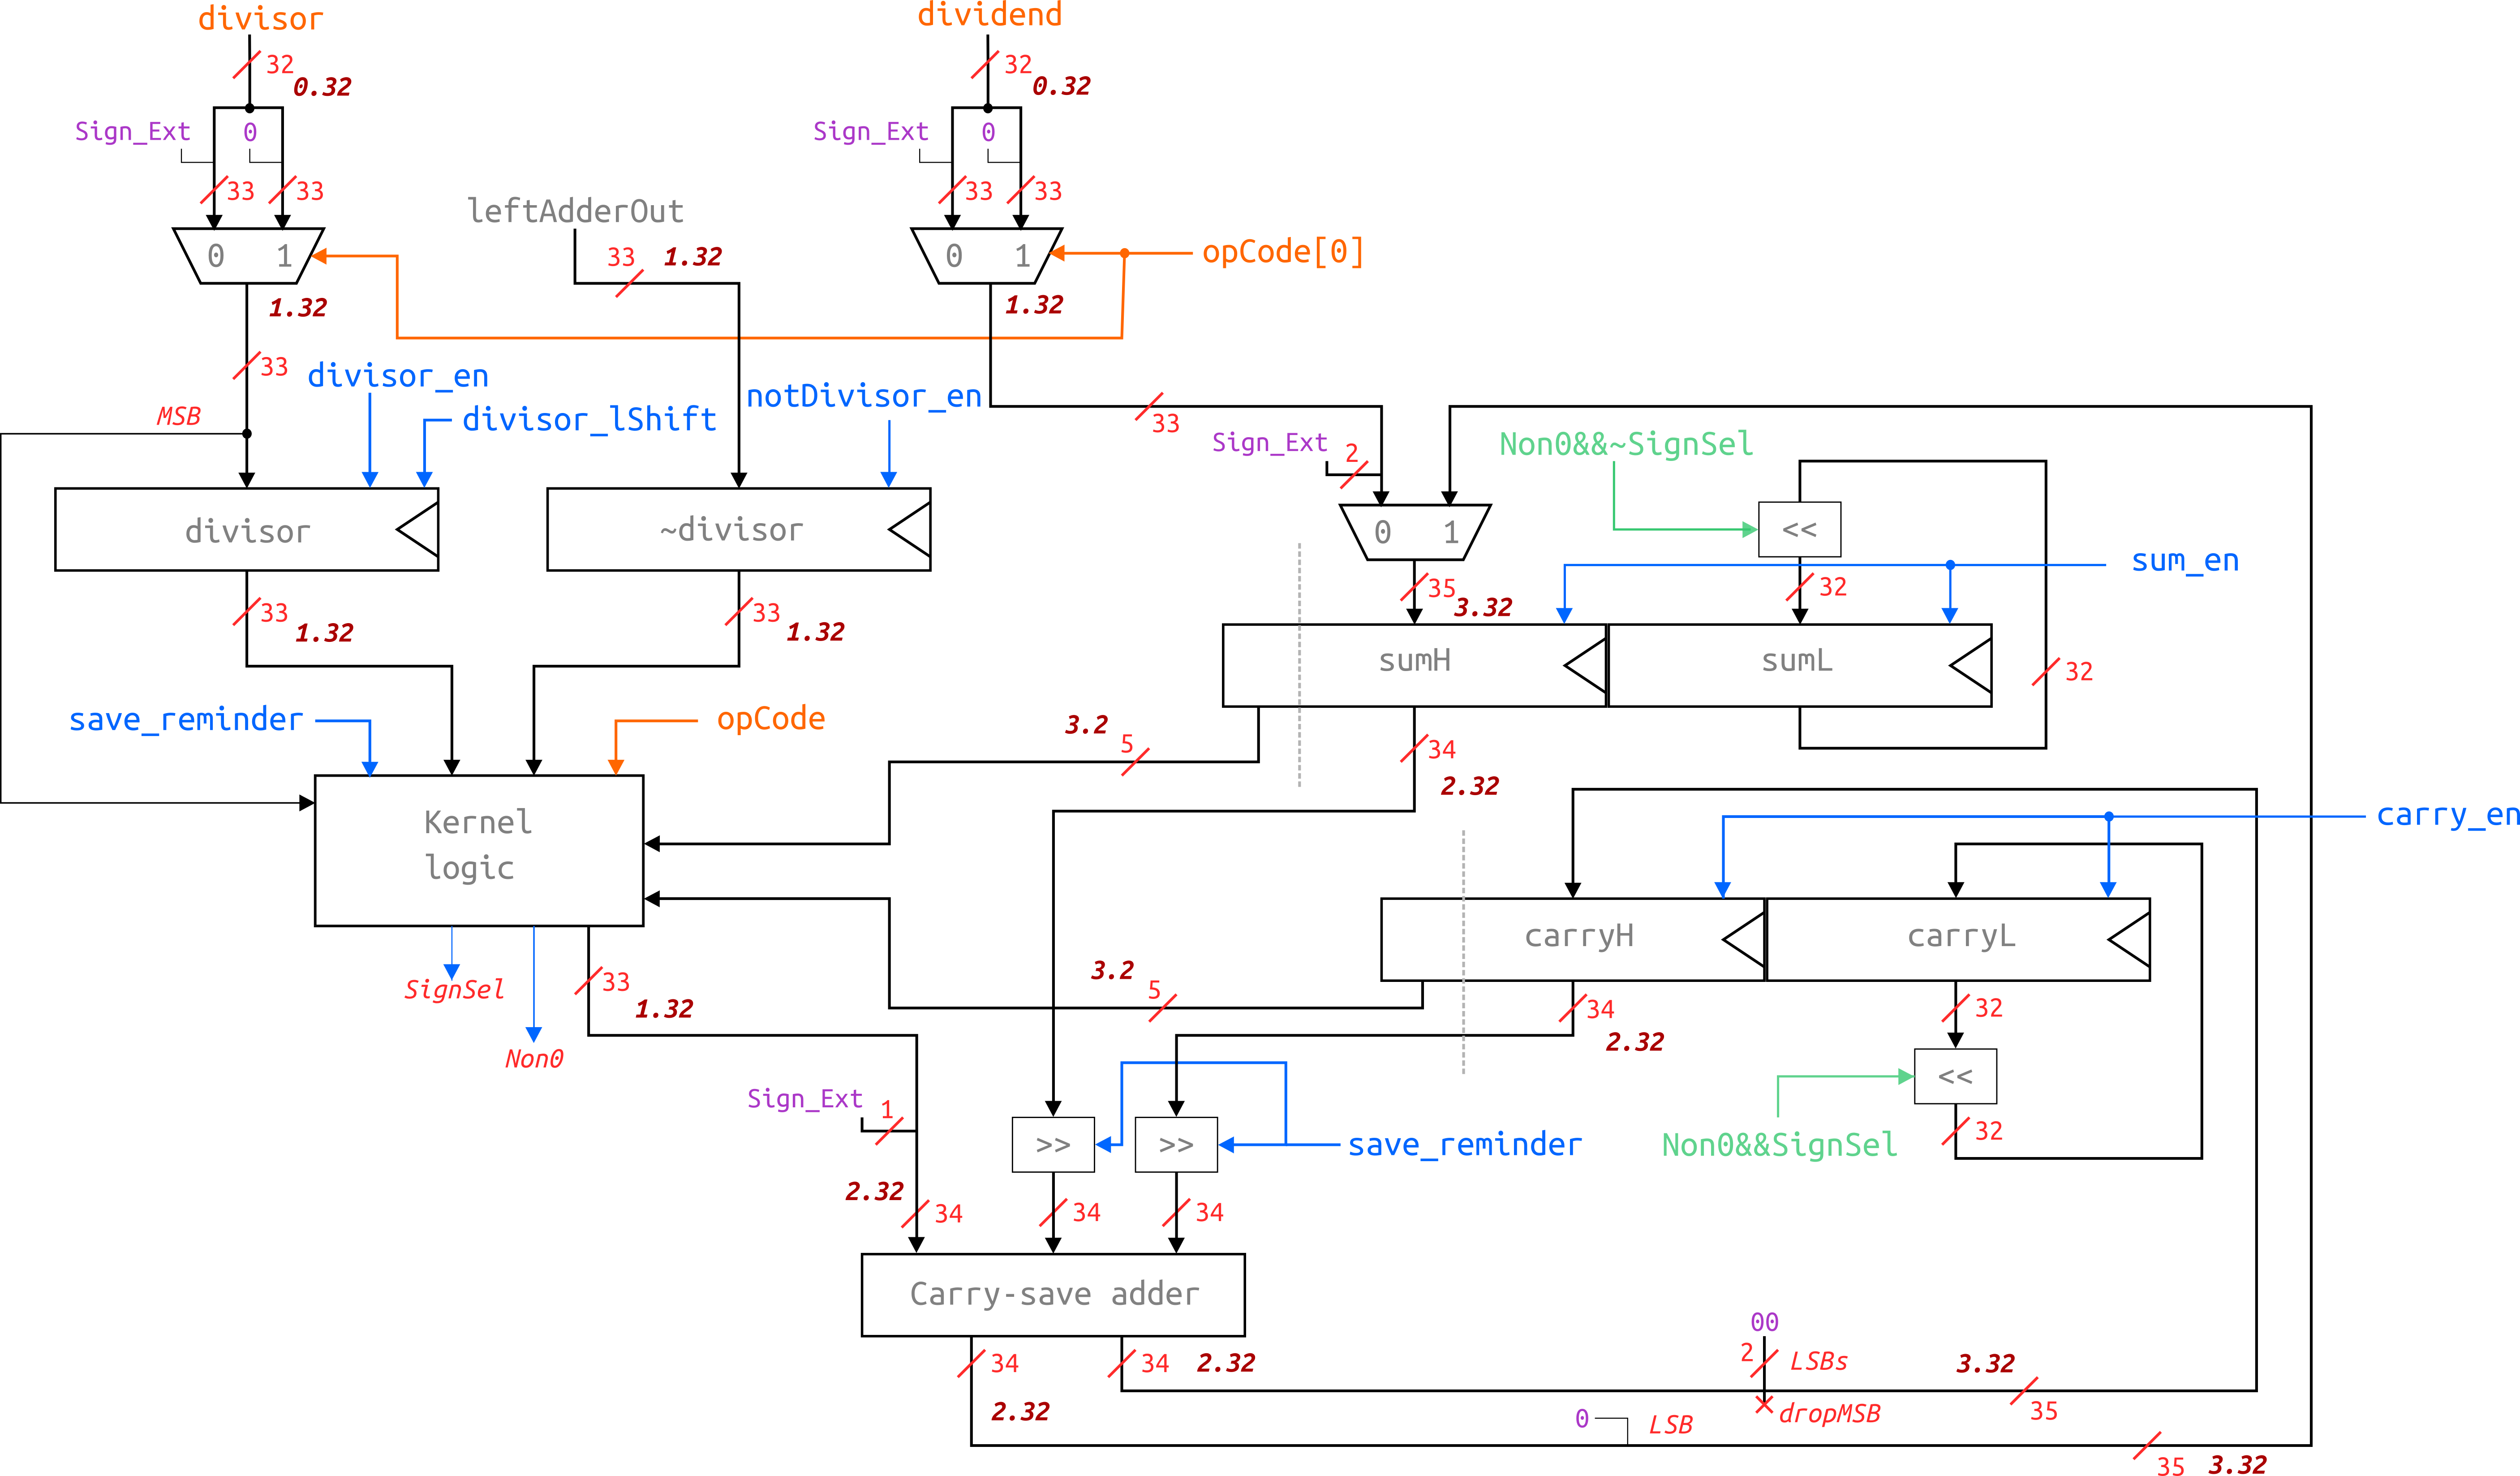
\includegraphics[angle=90,scale=0.9]{pics/divisorKernelLogic.png}
    \caption{Divisor upper datapath}
    \label{fig:my_label}
\end{figure}
\begin{figure}[H]
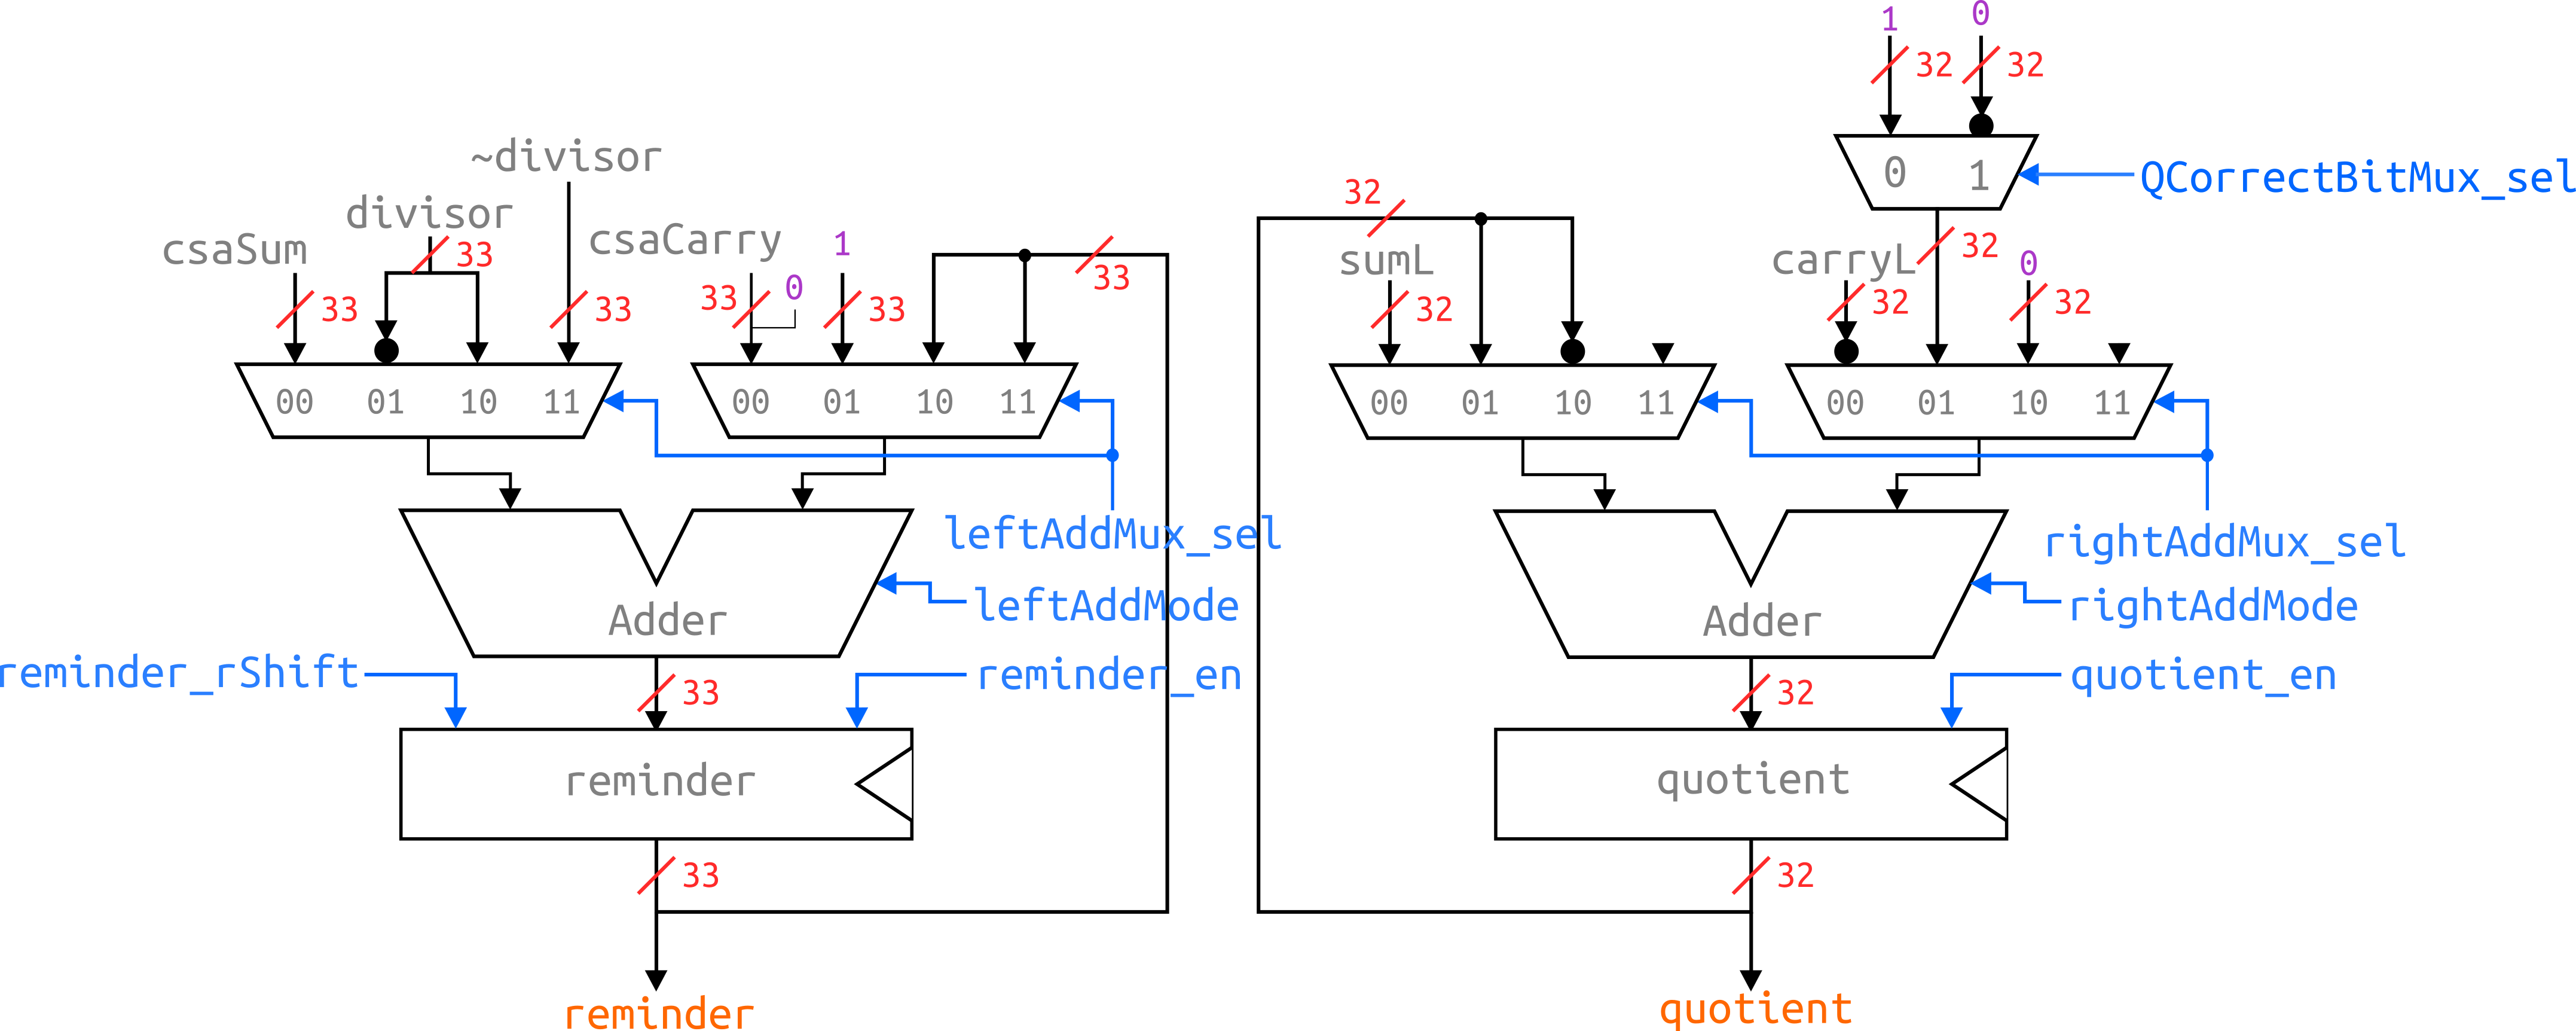
\includegraphics[scale=0.85]{pics/divisorOutputAdders.png}
    \caption{Divisor lower datapath}
    \label{fig:my_label}
\end{figure}
\begin{figure}[H]
\centering
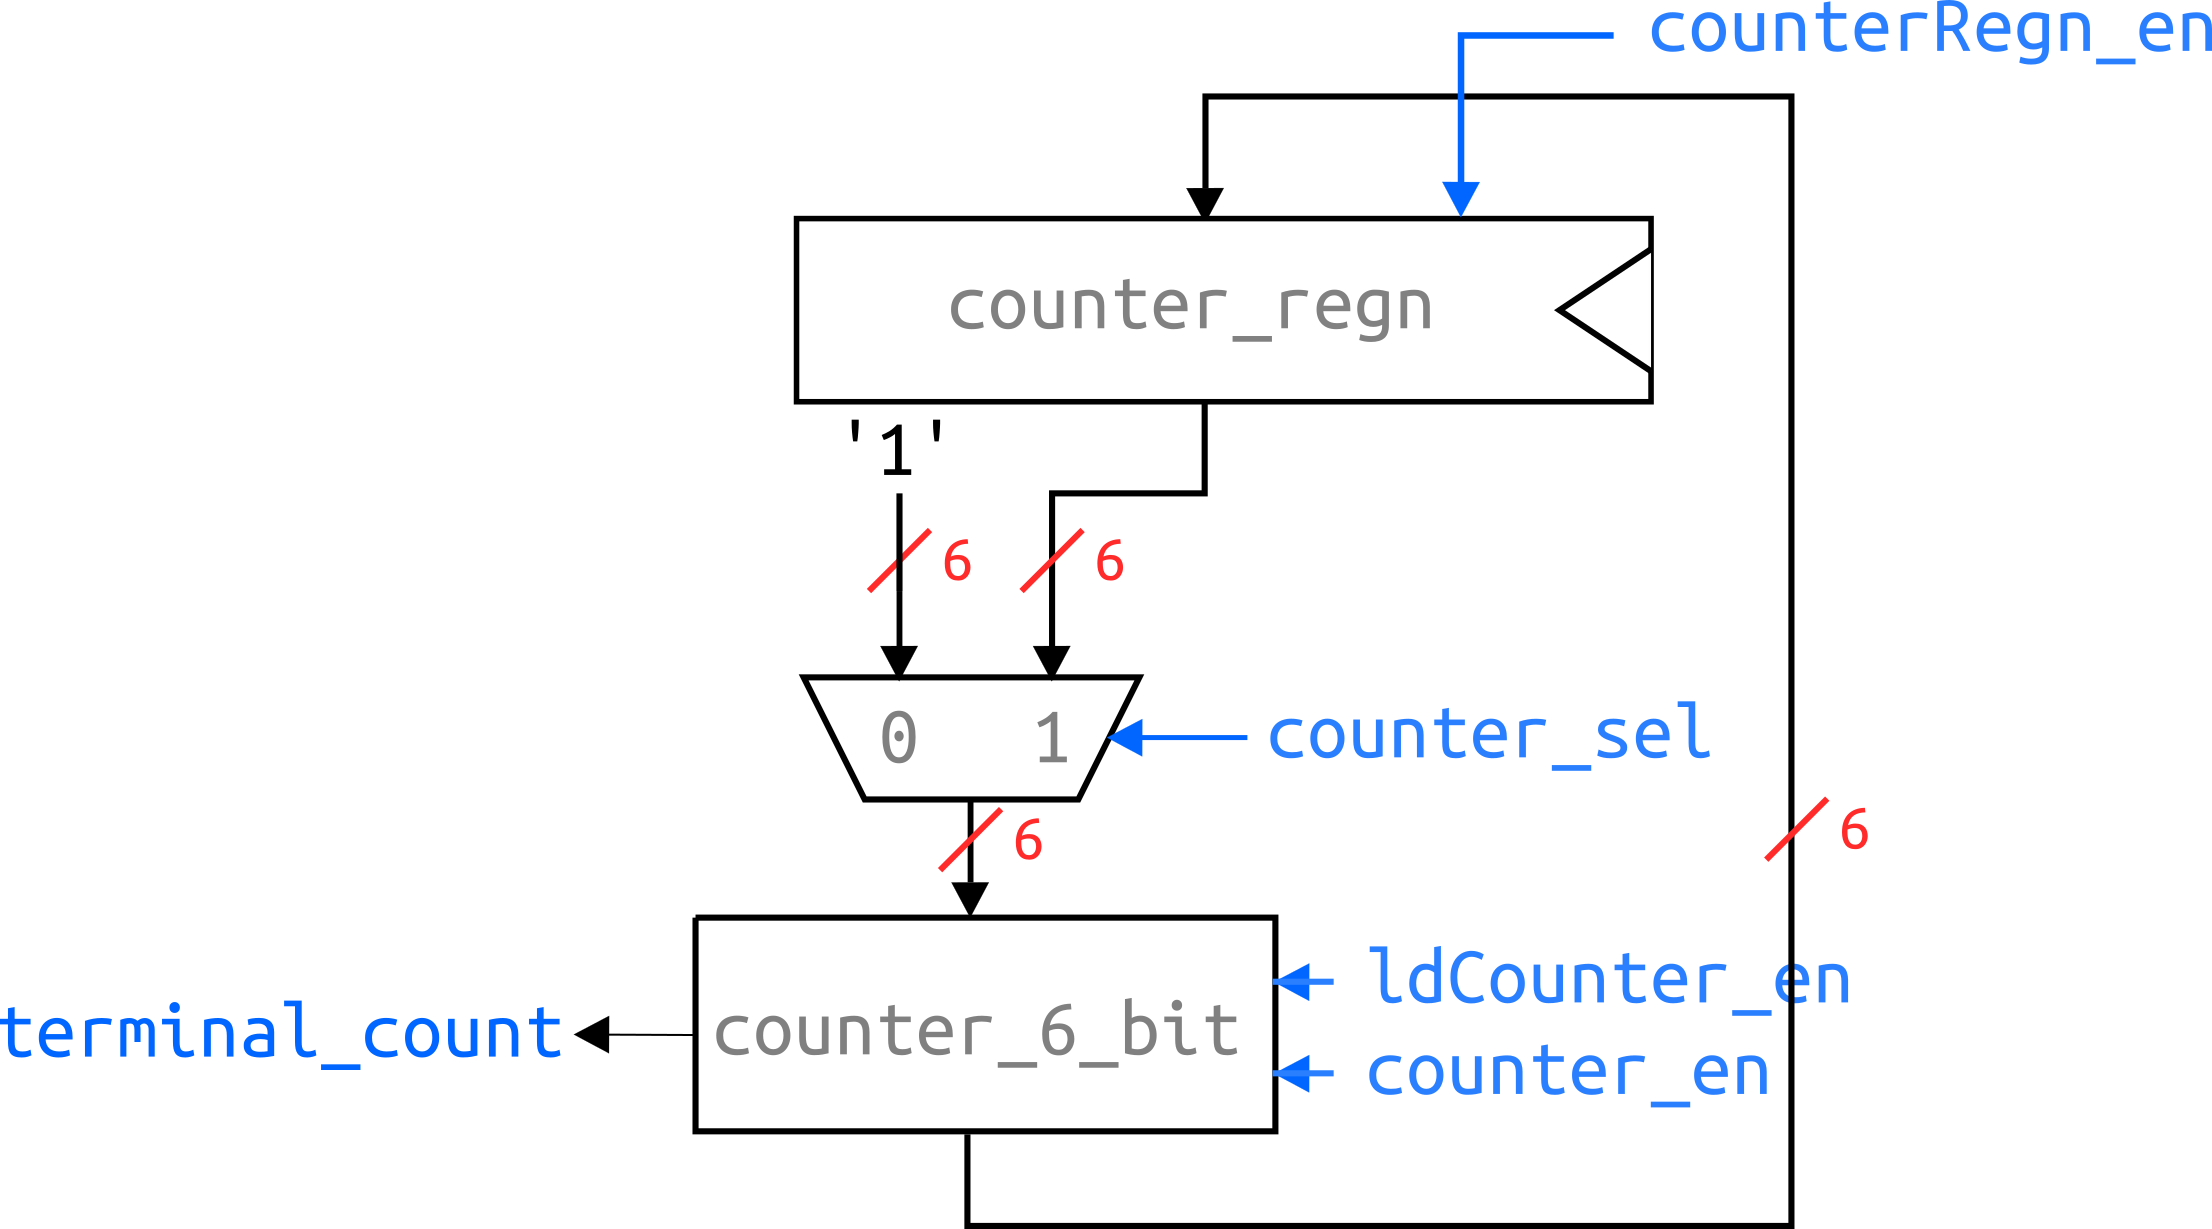
\includegraphics[scale=0.85]{pics/divisorCounter.png}
    \caption{Divisor counter}
    \label{fig:my_label}
\end{figure}
\subsubsection{Finite State Machine}
Here is done a fast description of what is done in each state of the FSM. For what concerns the \textit{idle} state and the start timing please check the multiplier section.
\paragraph{\textit{idle} State}
The machine waits for a rising edge on the start signal.
\paragraph{\textit{loadData} State}
Operands are loaded into the appropriate registers multiplied by 2. Divisor is checked on the fly to understand if it needs left shifts. In case it's ready, \textit{1} is loaded in the counter, since we need to perform just one step. This never verifies in case of signed division because $33^{rd}$ bit will always be a sign extension. 
\paragraph{\textit{divisorLShift} State}
Divisor is shifted and then a change of trend is checked by xoring $32^{nd}$ and $31^{st}$, since the shift will be updated in the successive cycle. The counter is enabled for counting how many kernel step must be performed, starting from 1 because divisor was loaded multiplied by 2.
\paragraph{\textit{saveIterloop} State}
Once the divisor is properly aligned it's important to keep track of how many multiplications by 2 have been done. Counter output is stored inside a dedicated feedback-register, the value will be read at the end few state later.
\paragraph{\textit{divKernelStep} State}
The main operation consists of a sum between the number produced by the proper logic and the previous partial reminder, expressed in sum-carry form. The result is automatically multiplied by two and feeds the registers in upper data path.\\
The two registers dedicated to the quotient also sample the new bit.
%può essere usato da due processori o due operazioni contemporaneamente contemporaneamente!
\paragraph{\textit{computeQ} State}
From now on only the two output adder are going to be used. Firstly they are set to compute a early version of the quotient and the reminder, the results will be then stored in the output registers used as accumulators. In this state the counter is re loaded with the previously store numeber of total shifts.
\paragraph{\textit{waitSignals} State}
Since the logic for the new state selection is driven from the output of the output, a clock cycle must be lost to let the signals propagate across the circuit. 
\paragraph{\textit{qInv} State}
Before going ahead, the sign of the quotient must be corrected. If the divisor is negative we must switch the sign performing the 2's complement of it's value.
\paragraph{\textit{correctDown} and \textit{correctUp} State}
These two states correct the results when needed.
\paragraph{\textit{RemCorrectio} State}
Lastly it's needed to shift right the reminder for a number of time that was stored in the counter in the \textit{computeQ} state. It must be noticed that the reminder is loaded already divided by 2 so, one step less is needed. For this purpose the shift register is made of 34 bits so that the actual least significant bit is not drop during last step.
\paragraph{\textit{divDone} State}
End of computation is signaled to the outer world.
\begin{figure}[H]
\centering
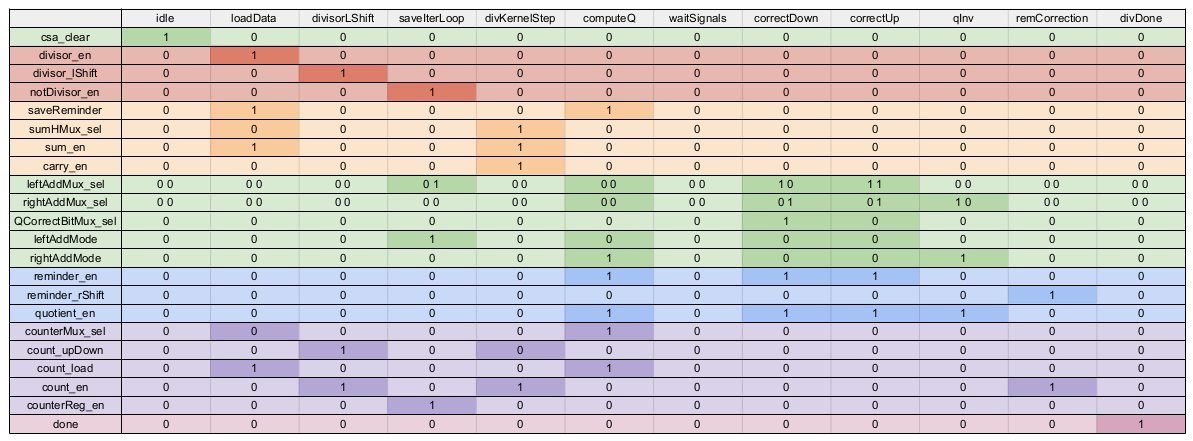
\includegraphics[scale=0.38]{pics/divControlTable.png}
    \caption{Divisor Control State Table}
    \label{fig:my_label}
\end{figure}
\begin{figure}[H]
\centering
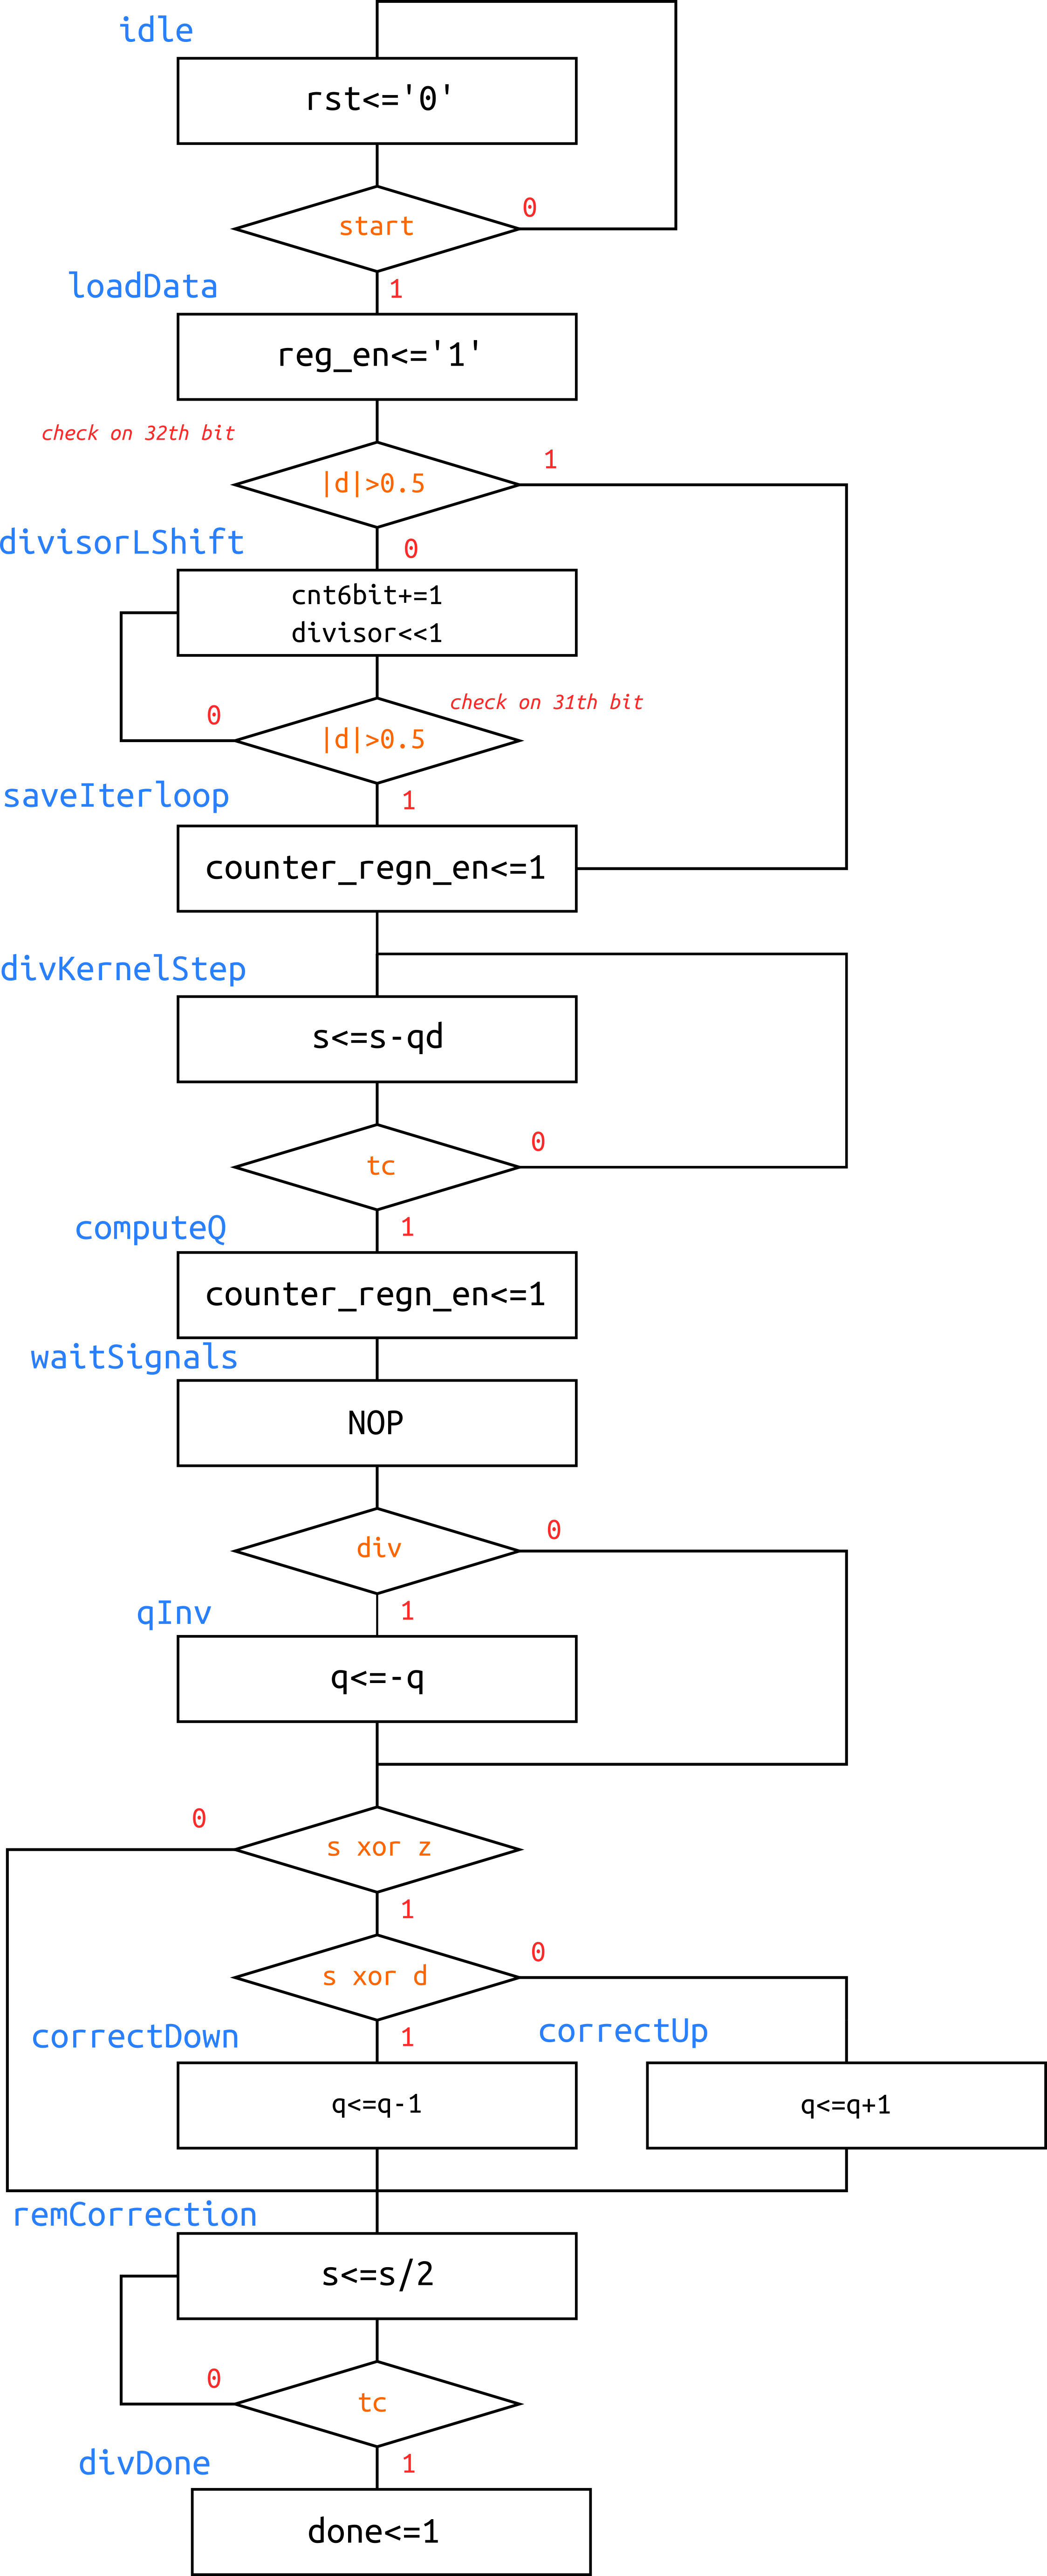
\includegraphics[scale=1]{pics/divisorASM.png}
    \caption{Divisor ASM}
    \label{fig:my_label}
\end{figure}
\subsection{Complete multiplication and division unit}
After the study of the single multiplication and division, it was not difficult to integrate everything in a single architecture.\\
Main difference is represented by a conditions checking circuit in which the following special case are tested:
\begin{itemize}
    \item Two consecutive instructions require the same computation, which is avoided and the result is directly given at the output.
    \item In case of division, divisor value is 0.
    \item In case of signed division, divisor value is -1 and dividend one is $-2^{k-1}$, so that the resulting quotient will overflow the capability of 32 bits.
\end{itemize}
\subsubsection{Datapath}
\begin{figure}[H]
\centering
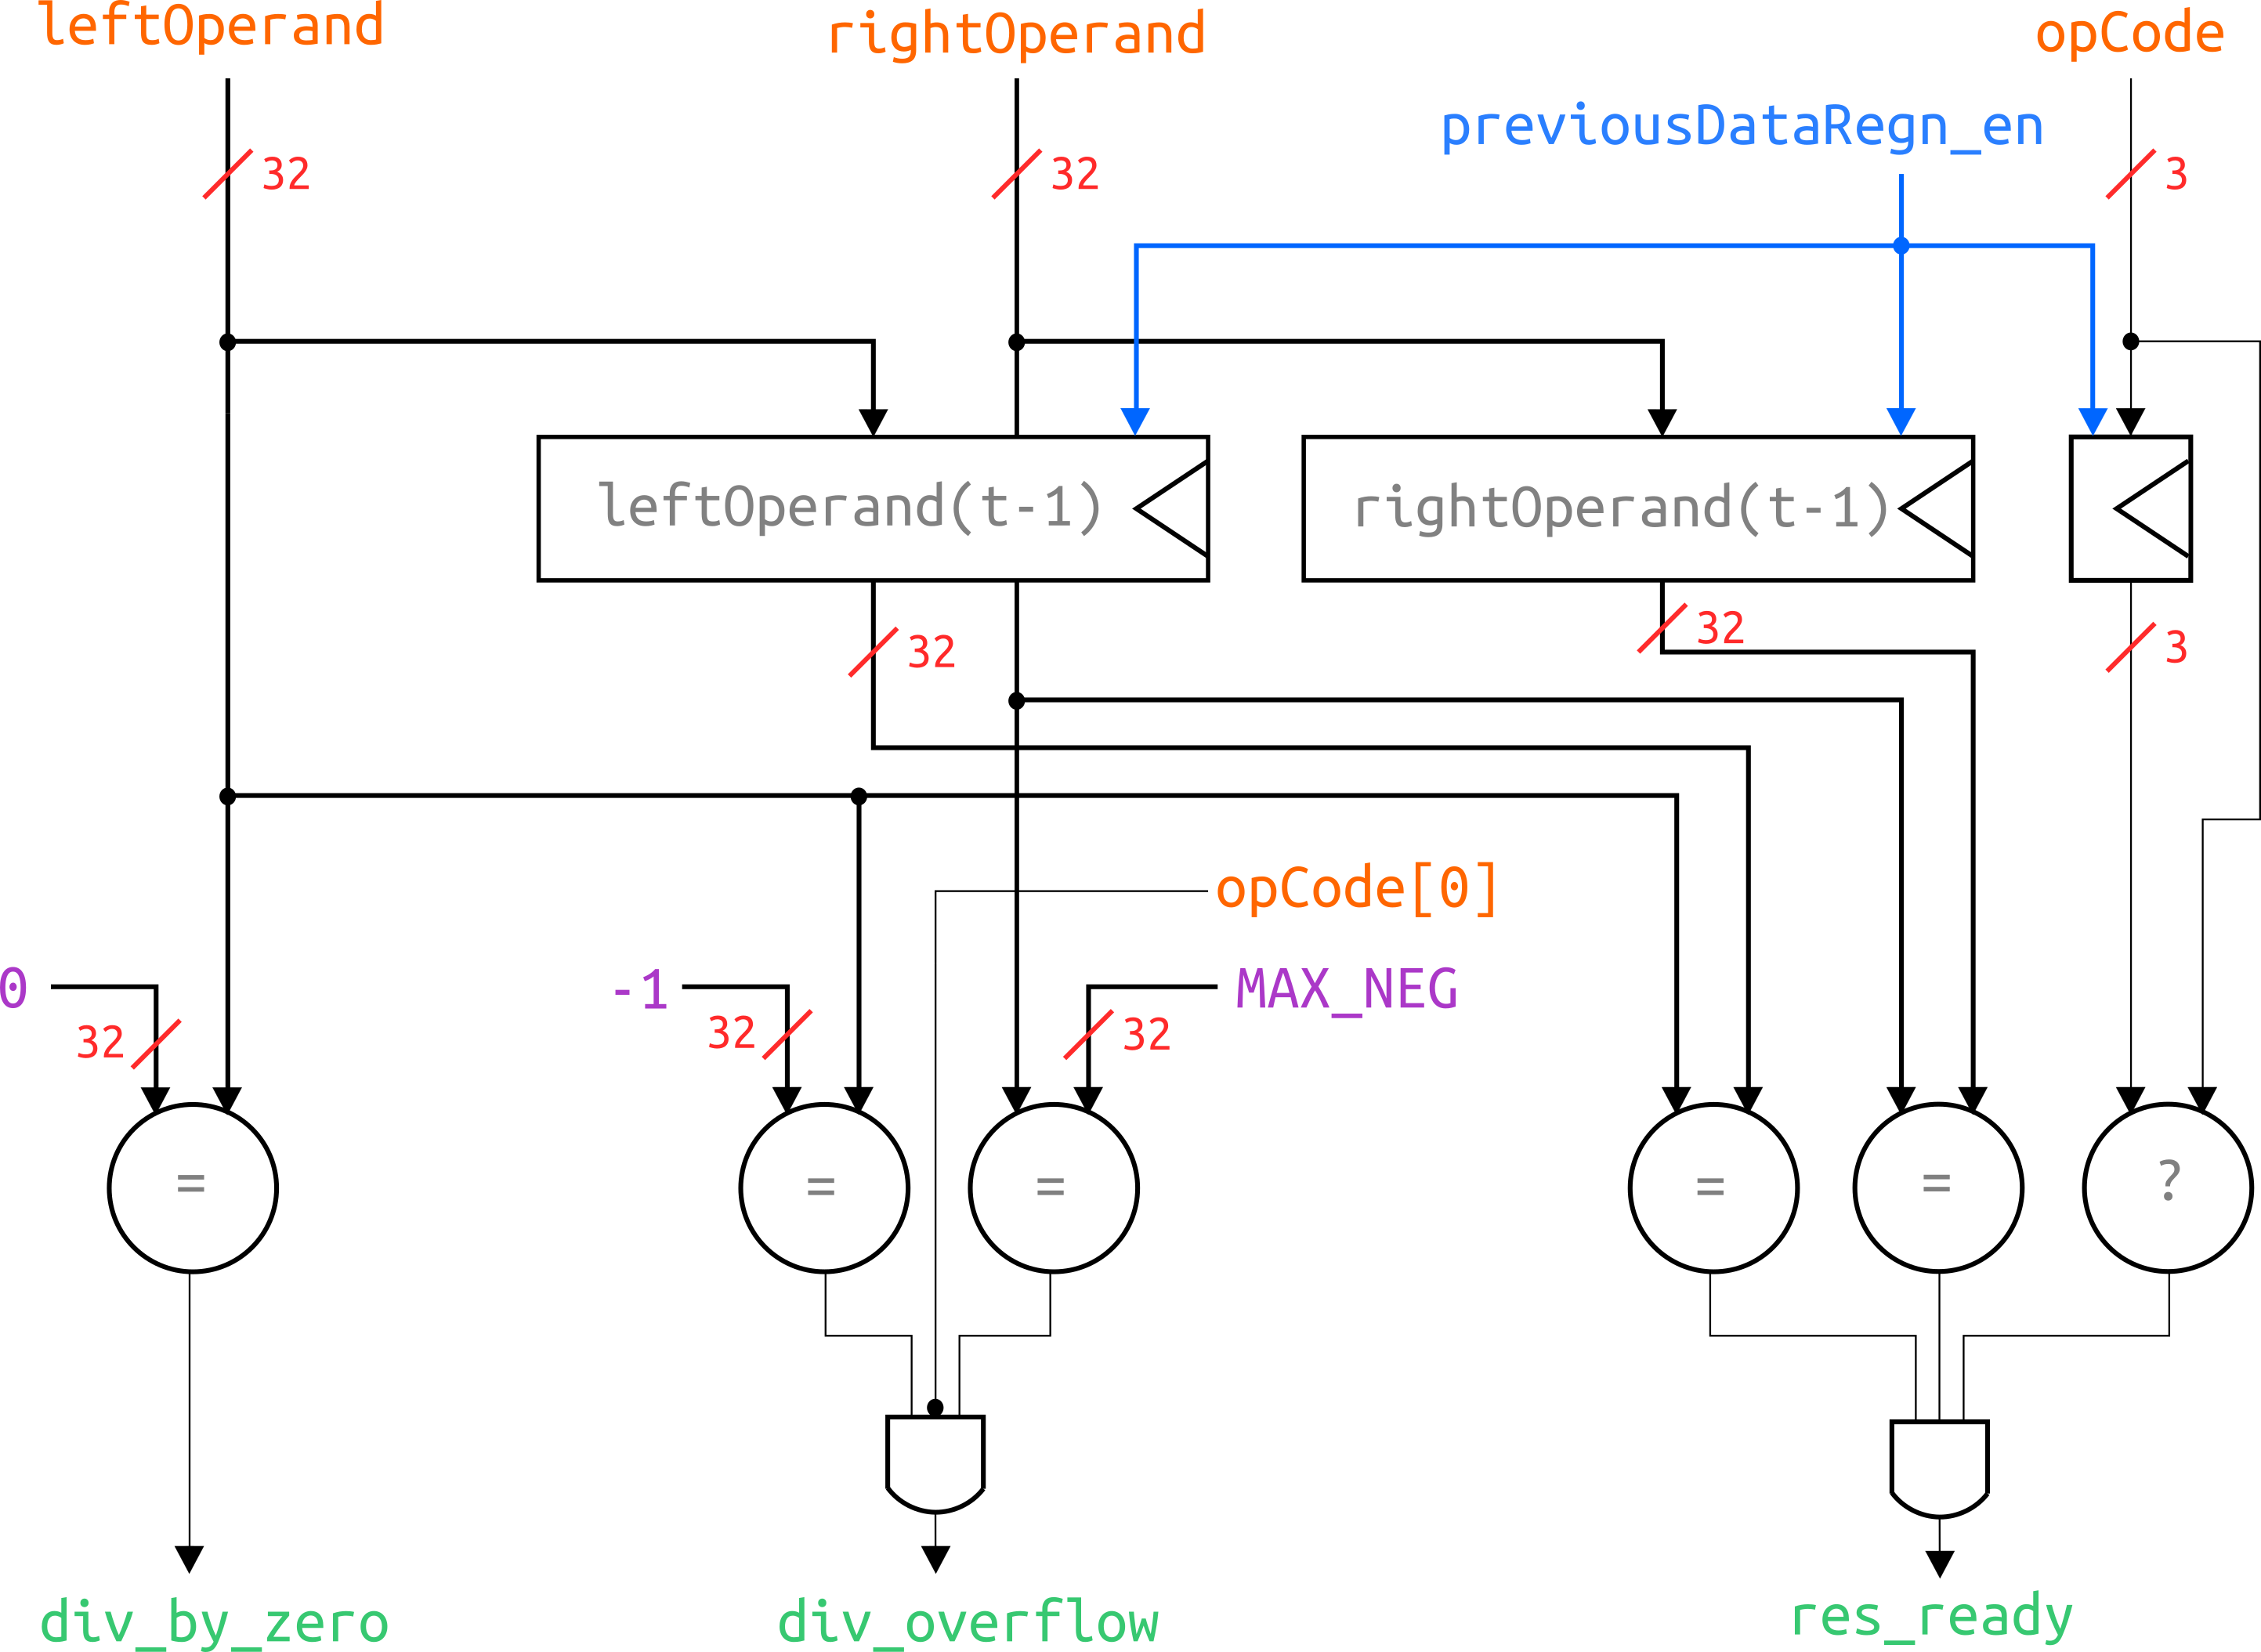
\includegraphics[scale=1]{pics/feedbackNet.png}
    \caption{Control net for special cases}
    \label{fig:my_label}
\end{figure}
\begin{figure}[H]
\centering
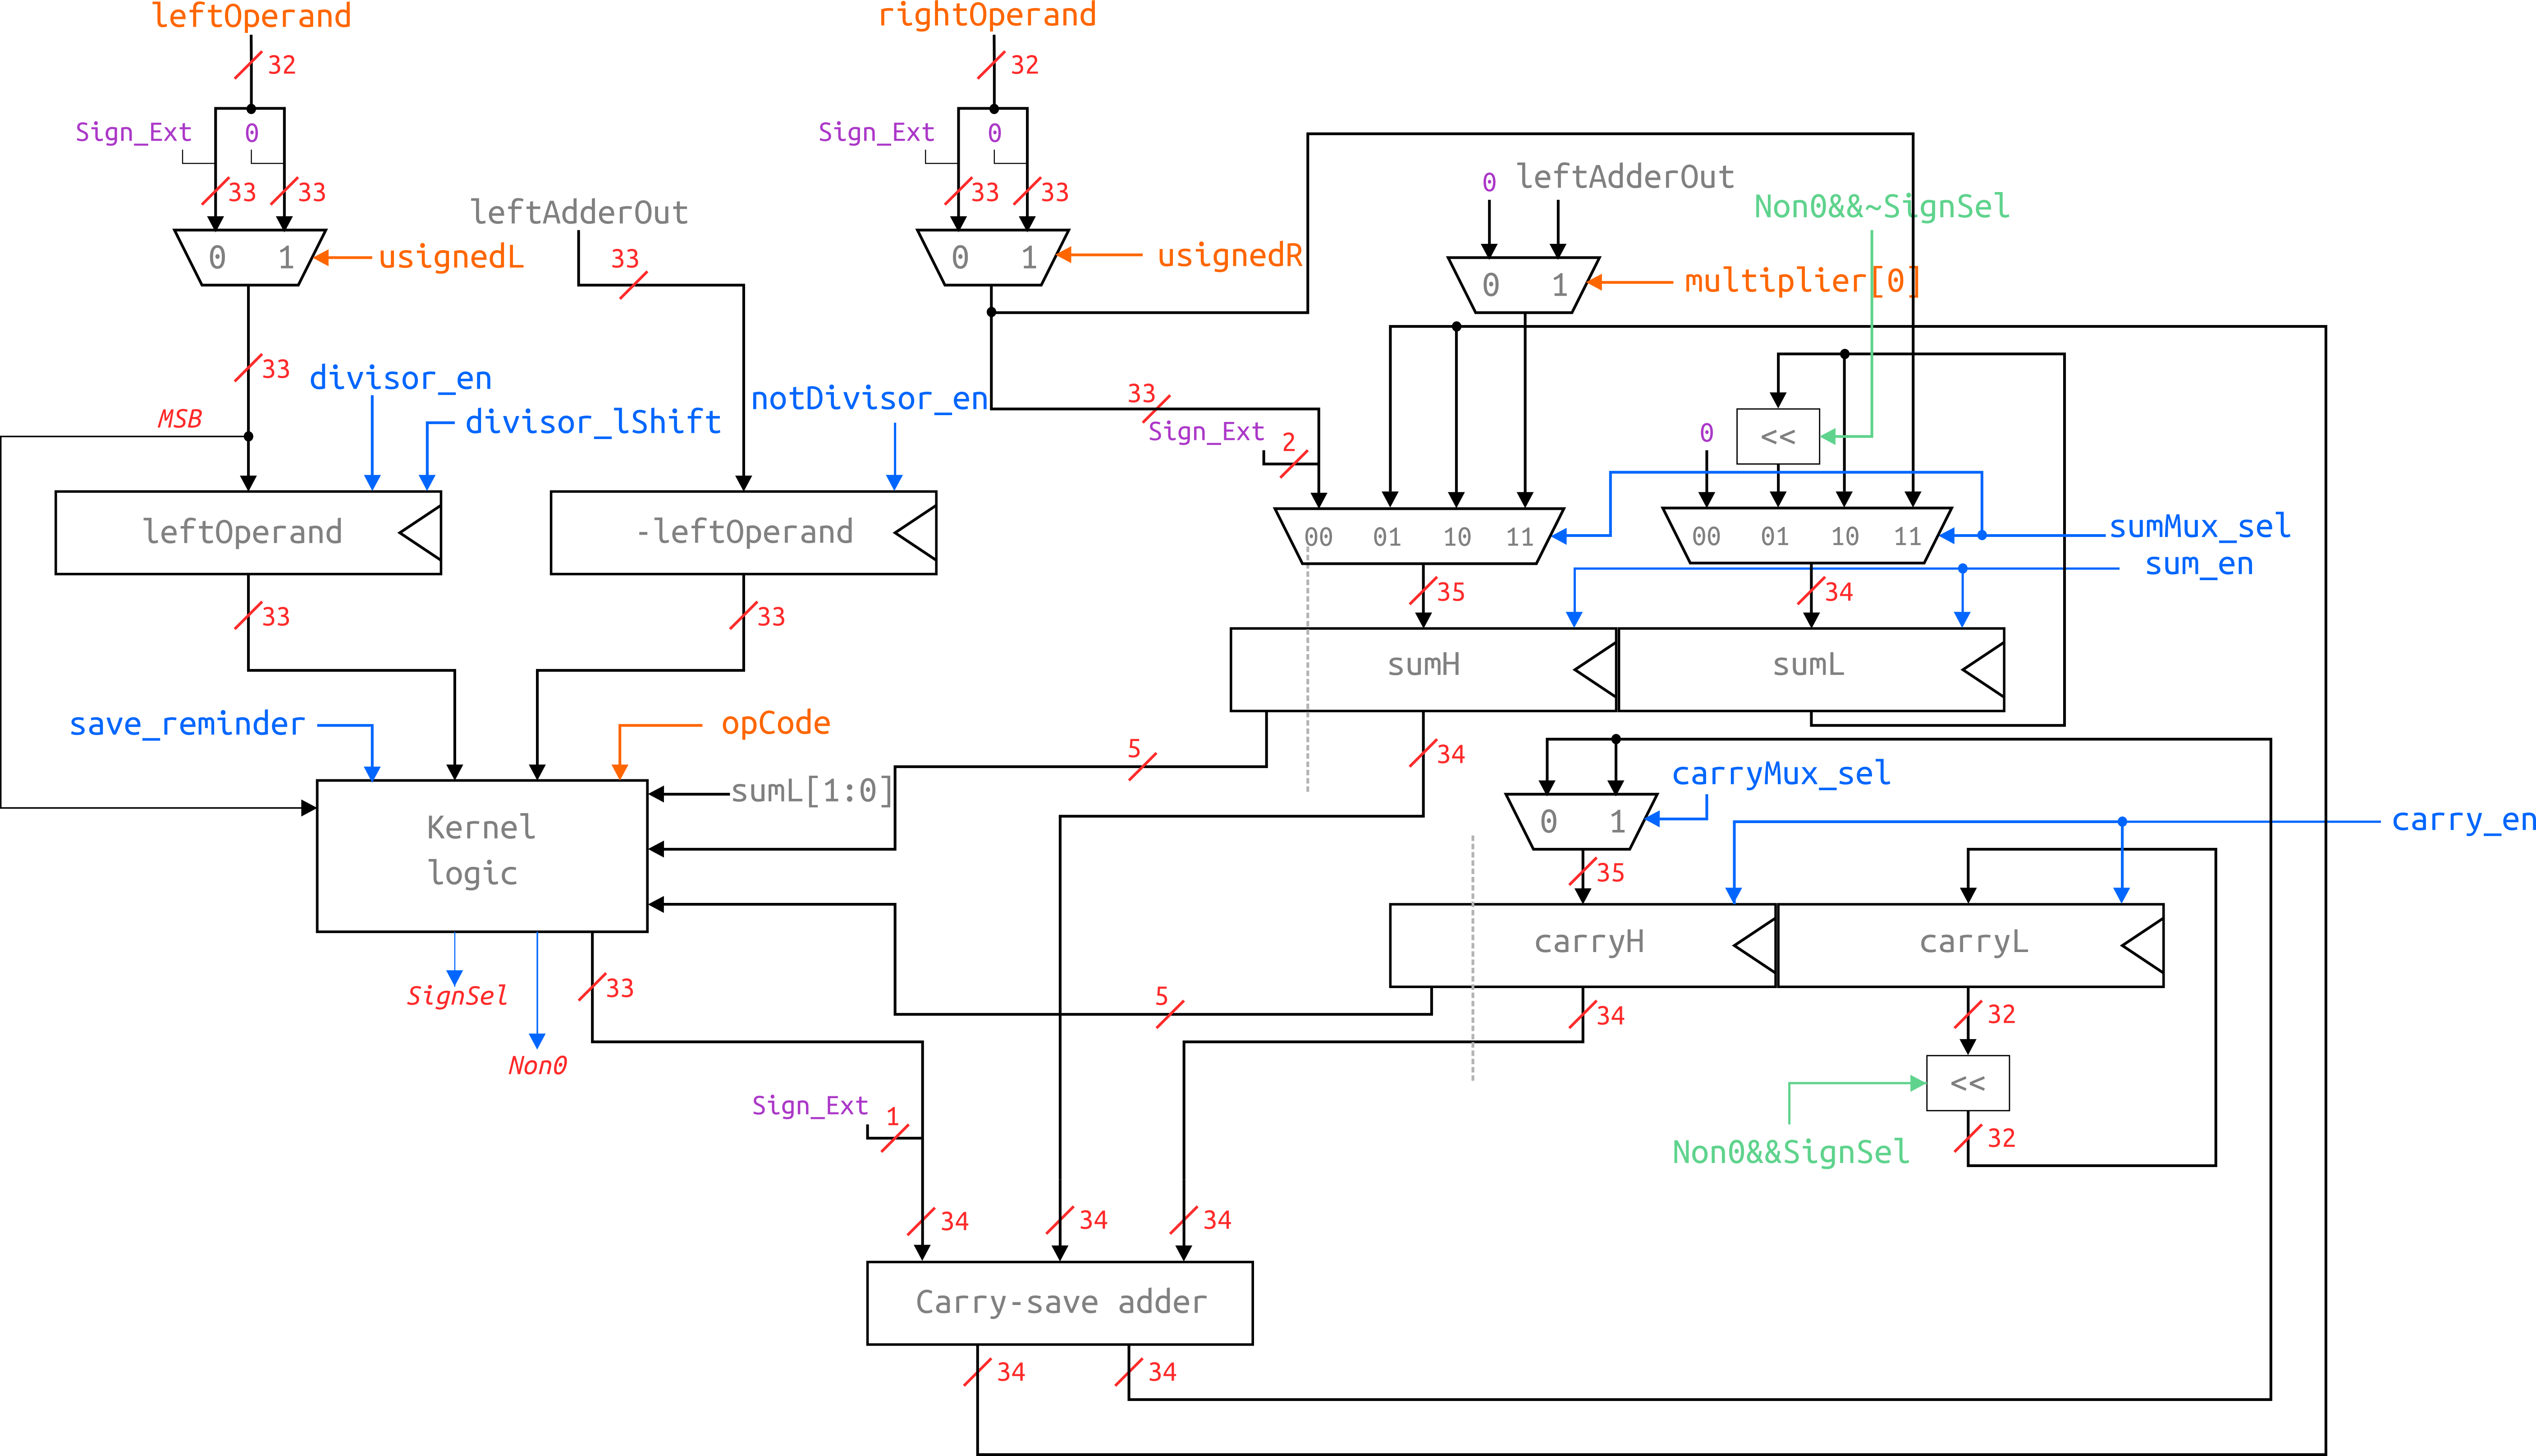
\includegraphics[angle=90,scale=1]{pics/kernelLogic.png}
    \caption{Upper data path}
    \label{fig:my_label}
\end{figure}
\begin{figure}[H]
\centering
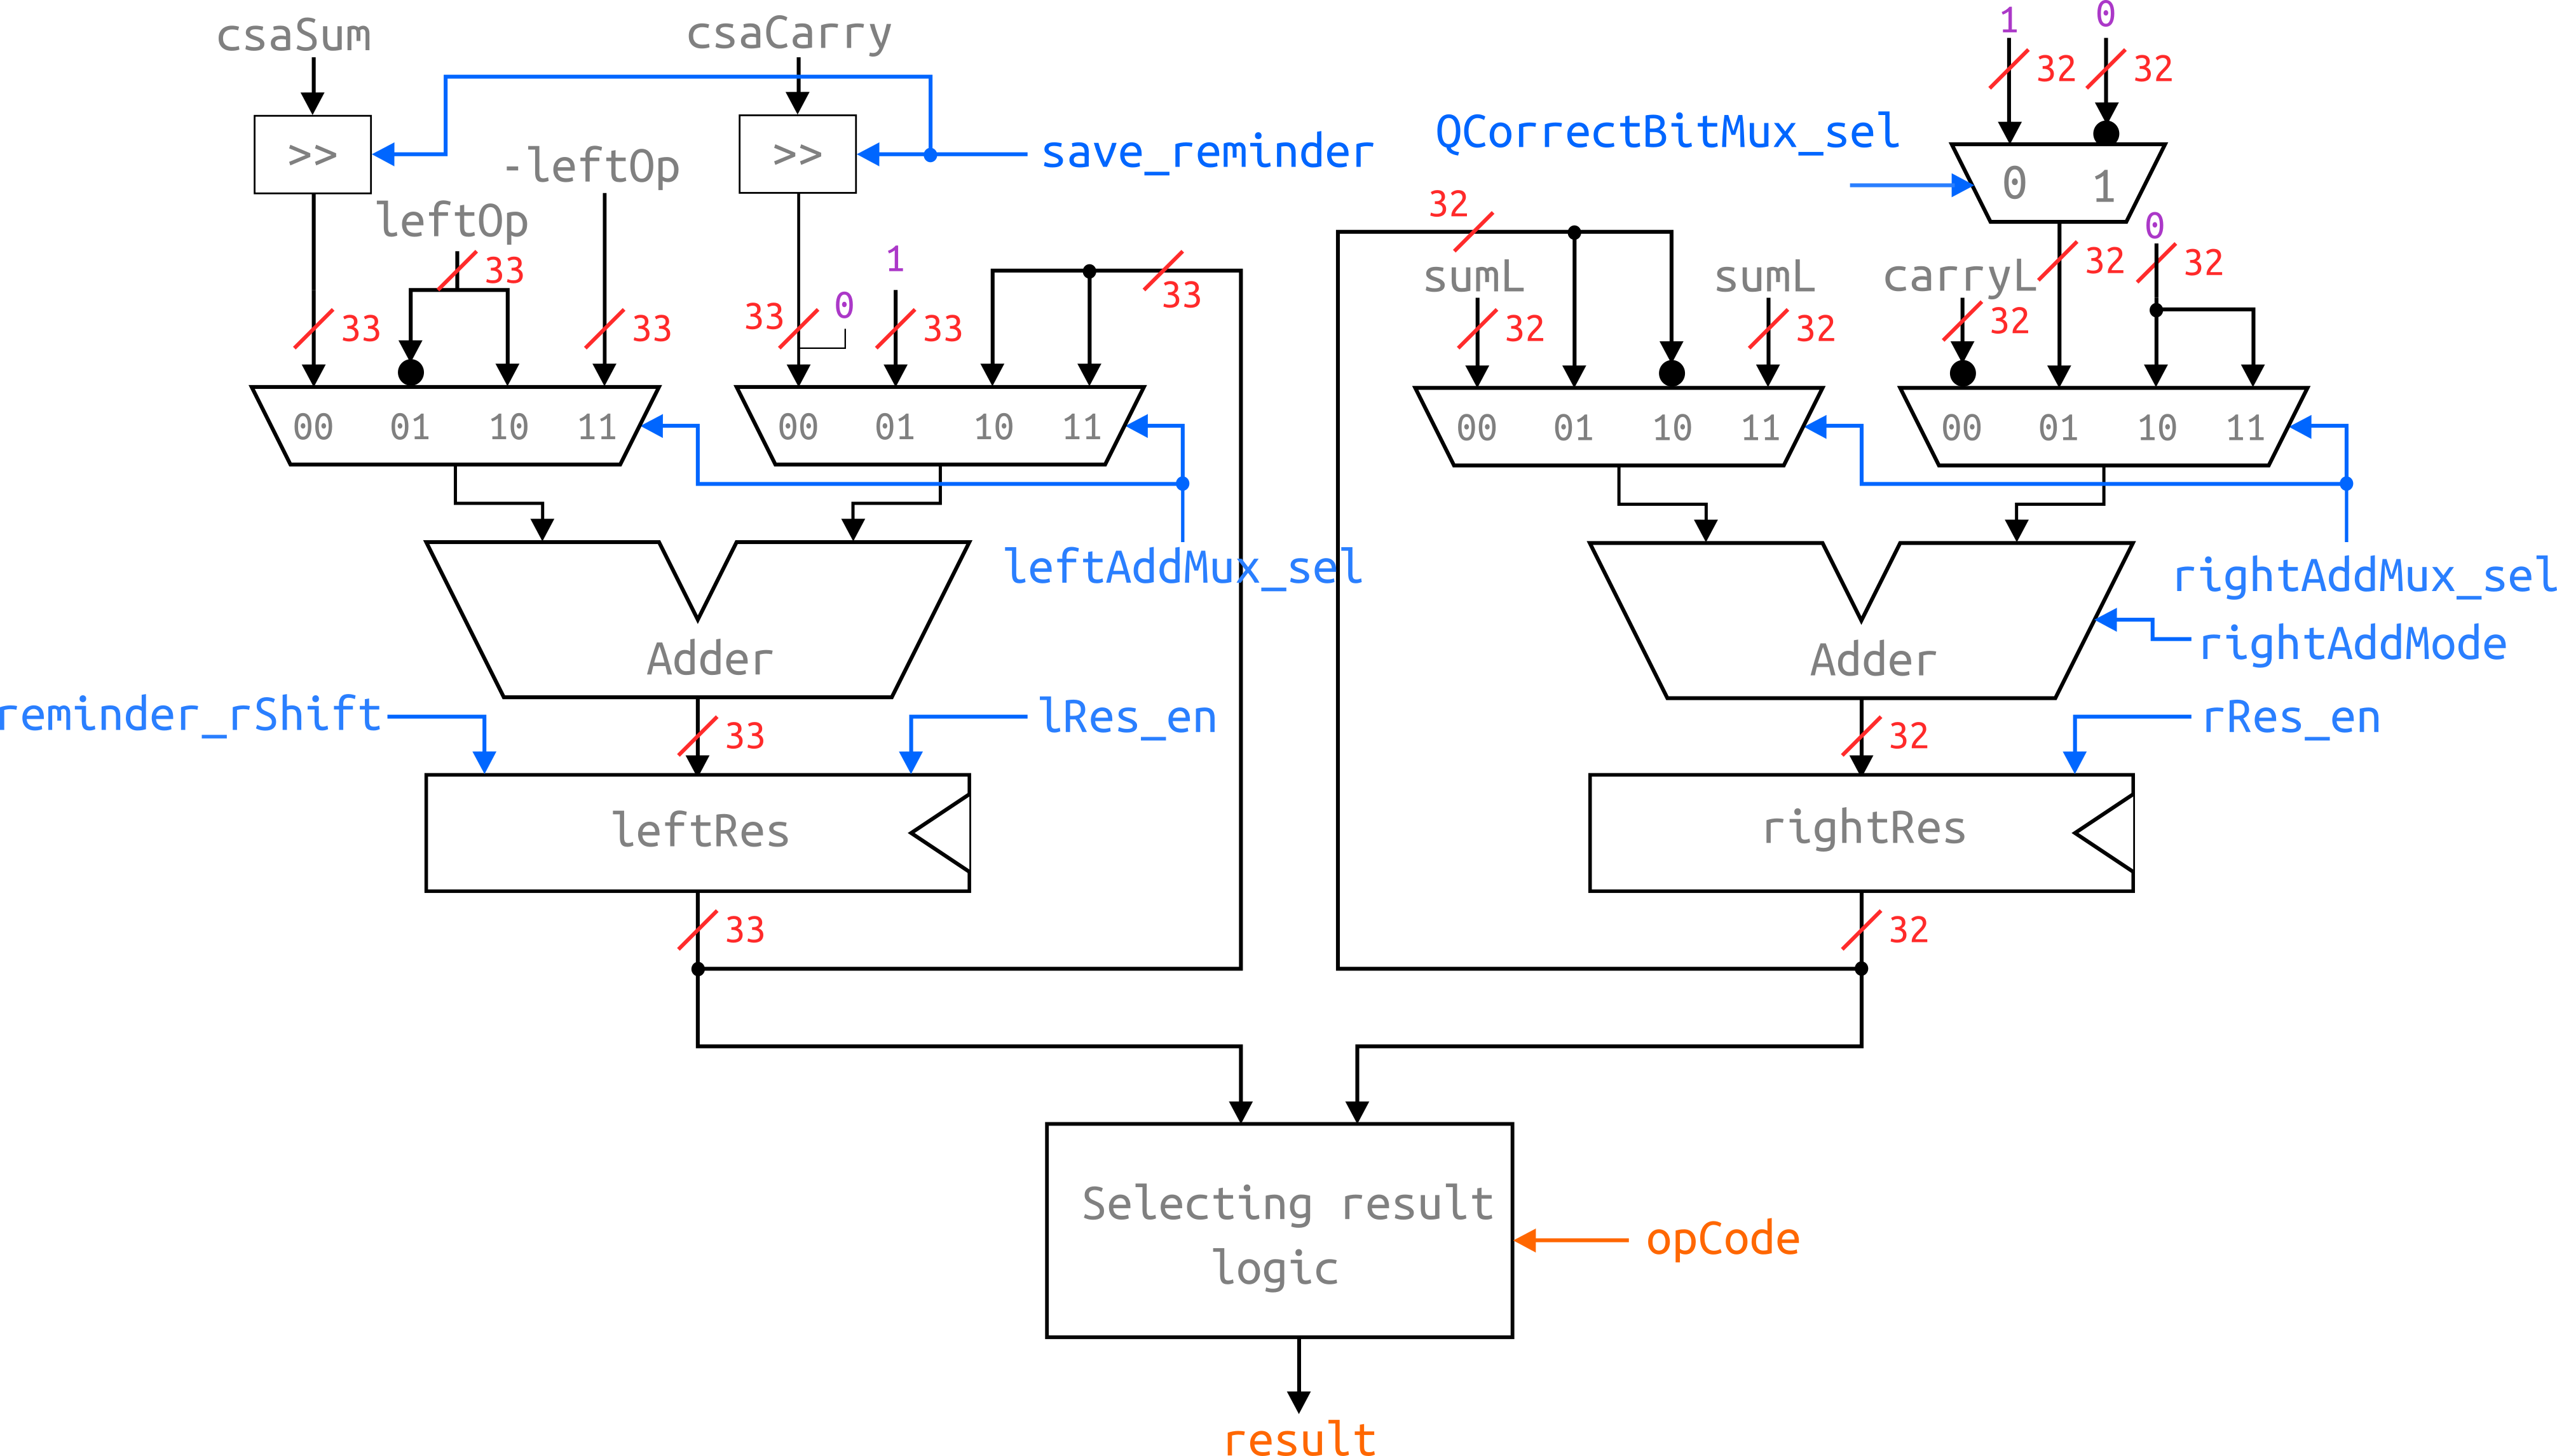
\includegraphics[scale=0.9]{pics/outputAdders.png}
    \caption{Lower data path}
    \label{fig:my_label}
\end{figure}
\begin{figure}[H]
\centering
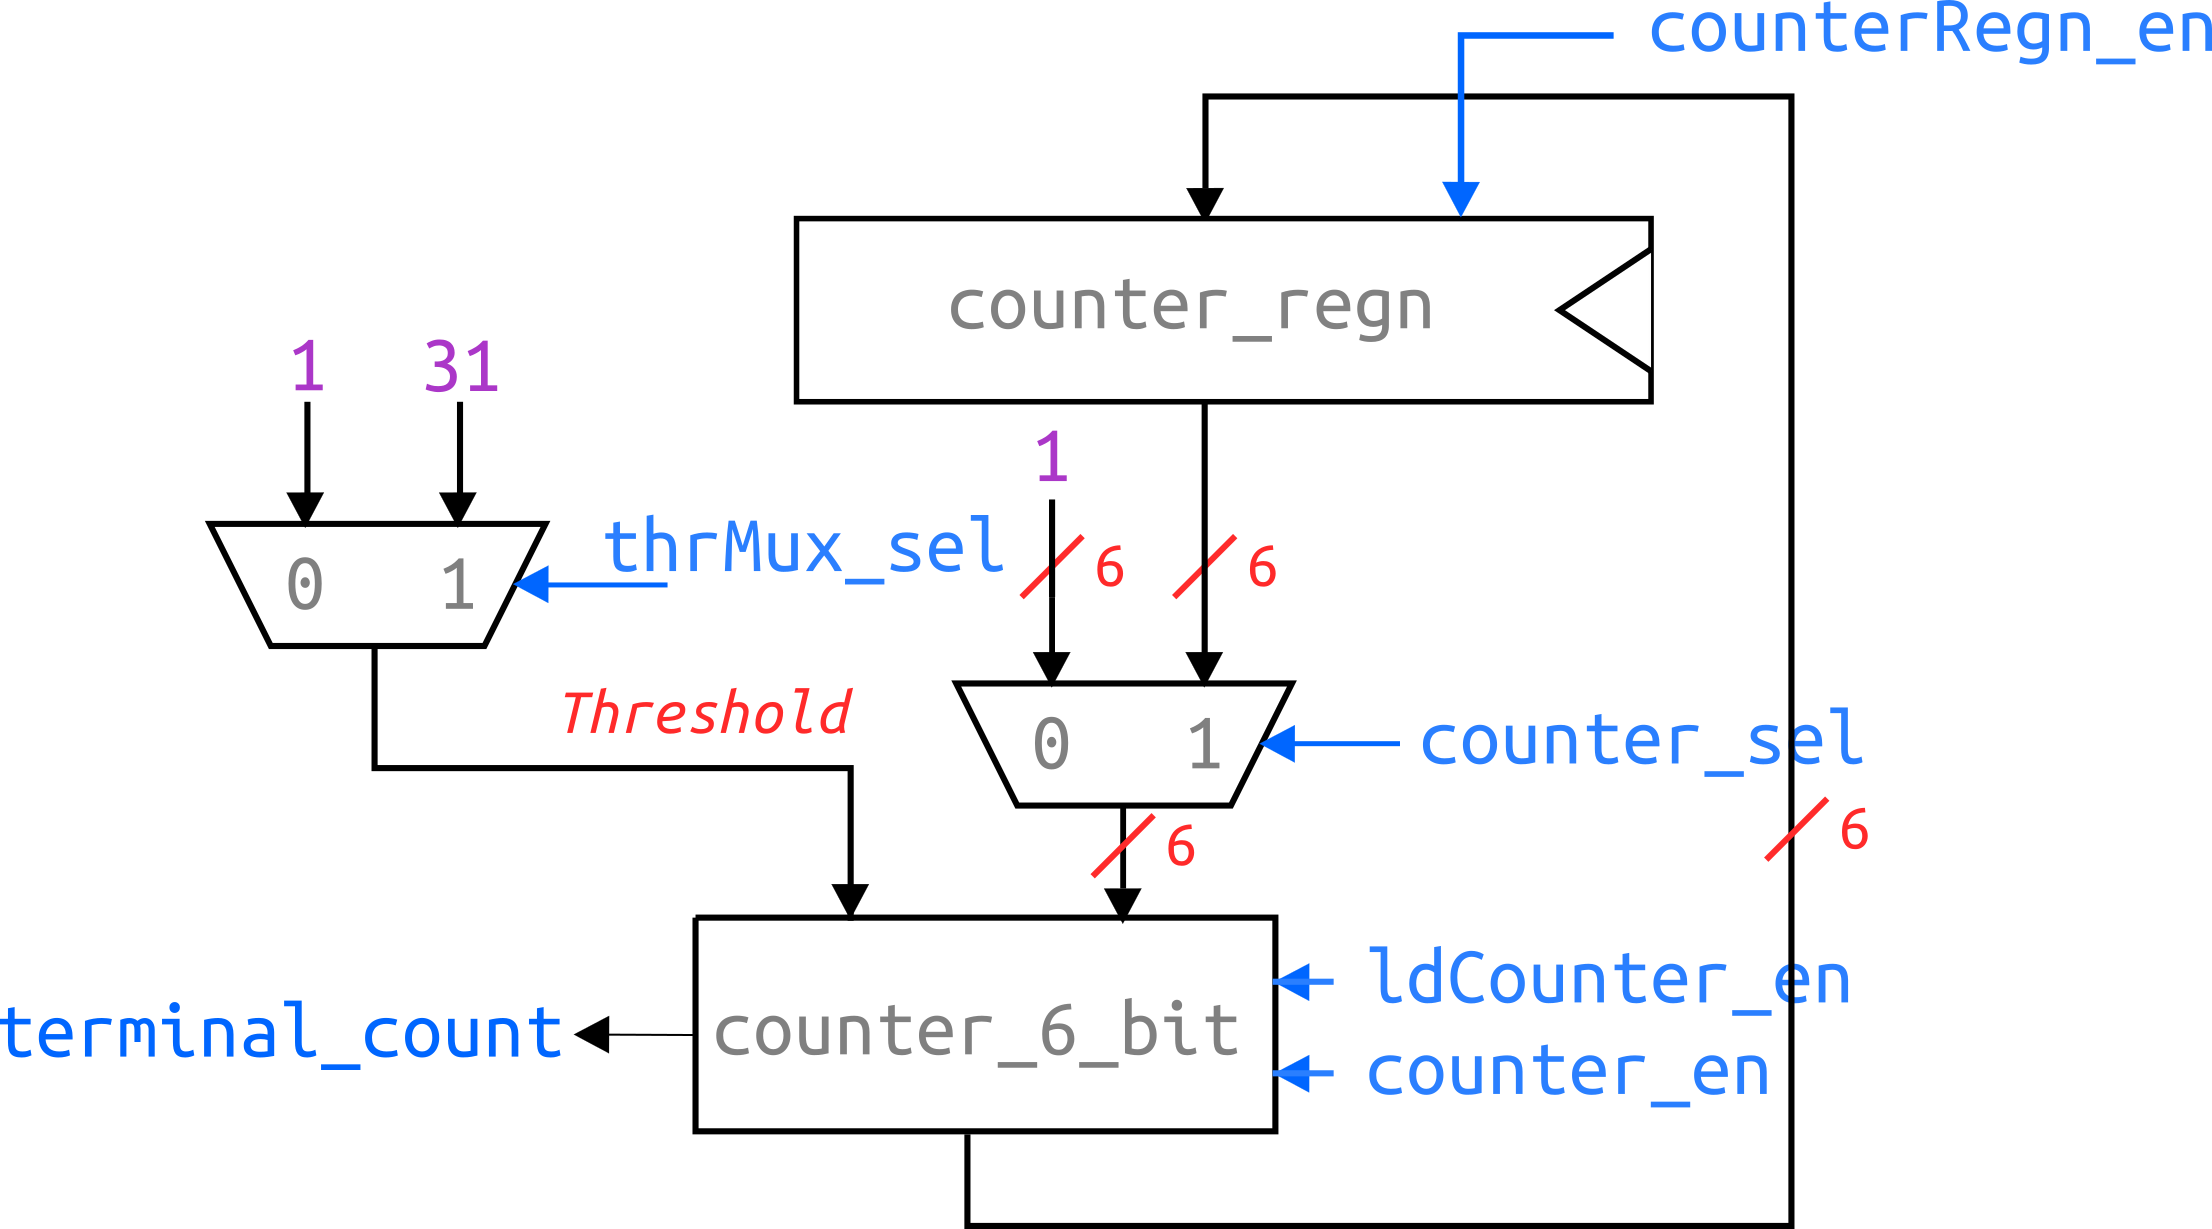
\includegraphics[scale=1]{pics/counter.png}
    \caption{Counter and related controls}
    \label{fig:my_label}
\end{figure}
\subsubsection{Finite State Machine}
\begin{figure}[H]
\centering
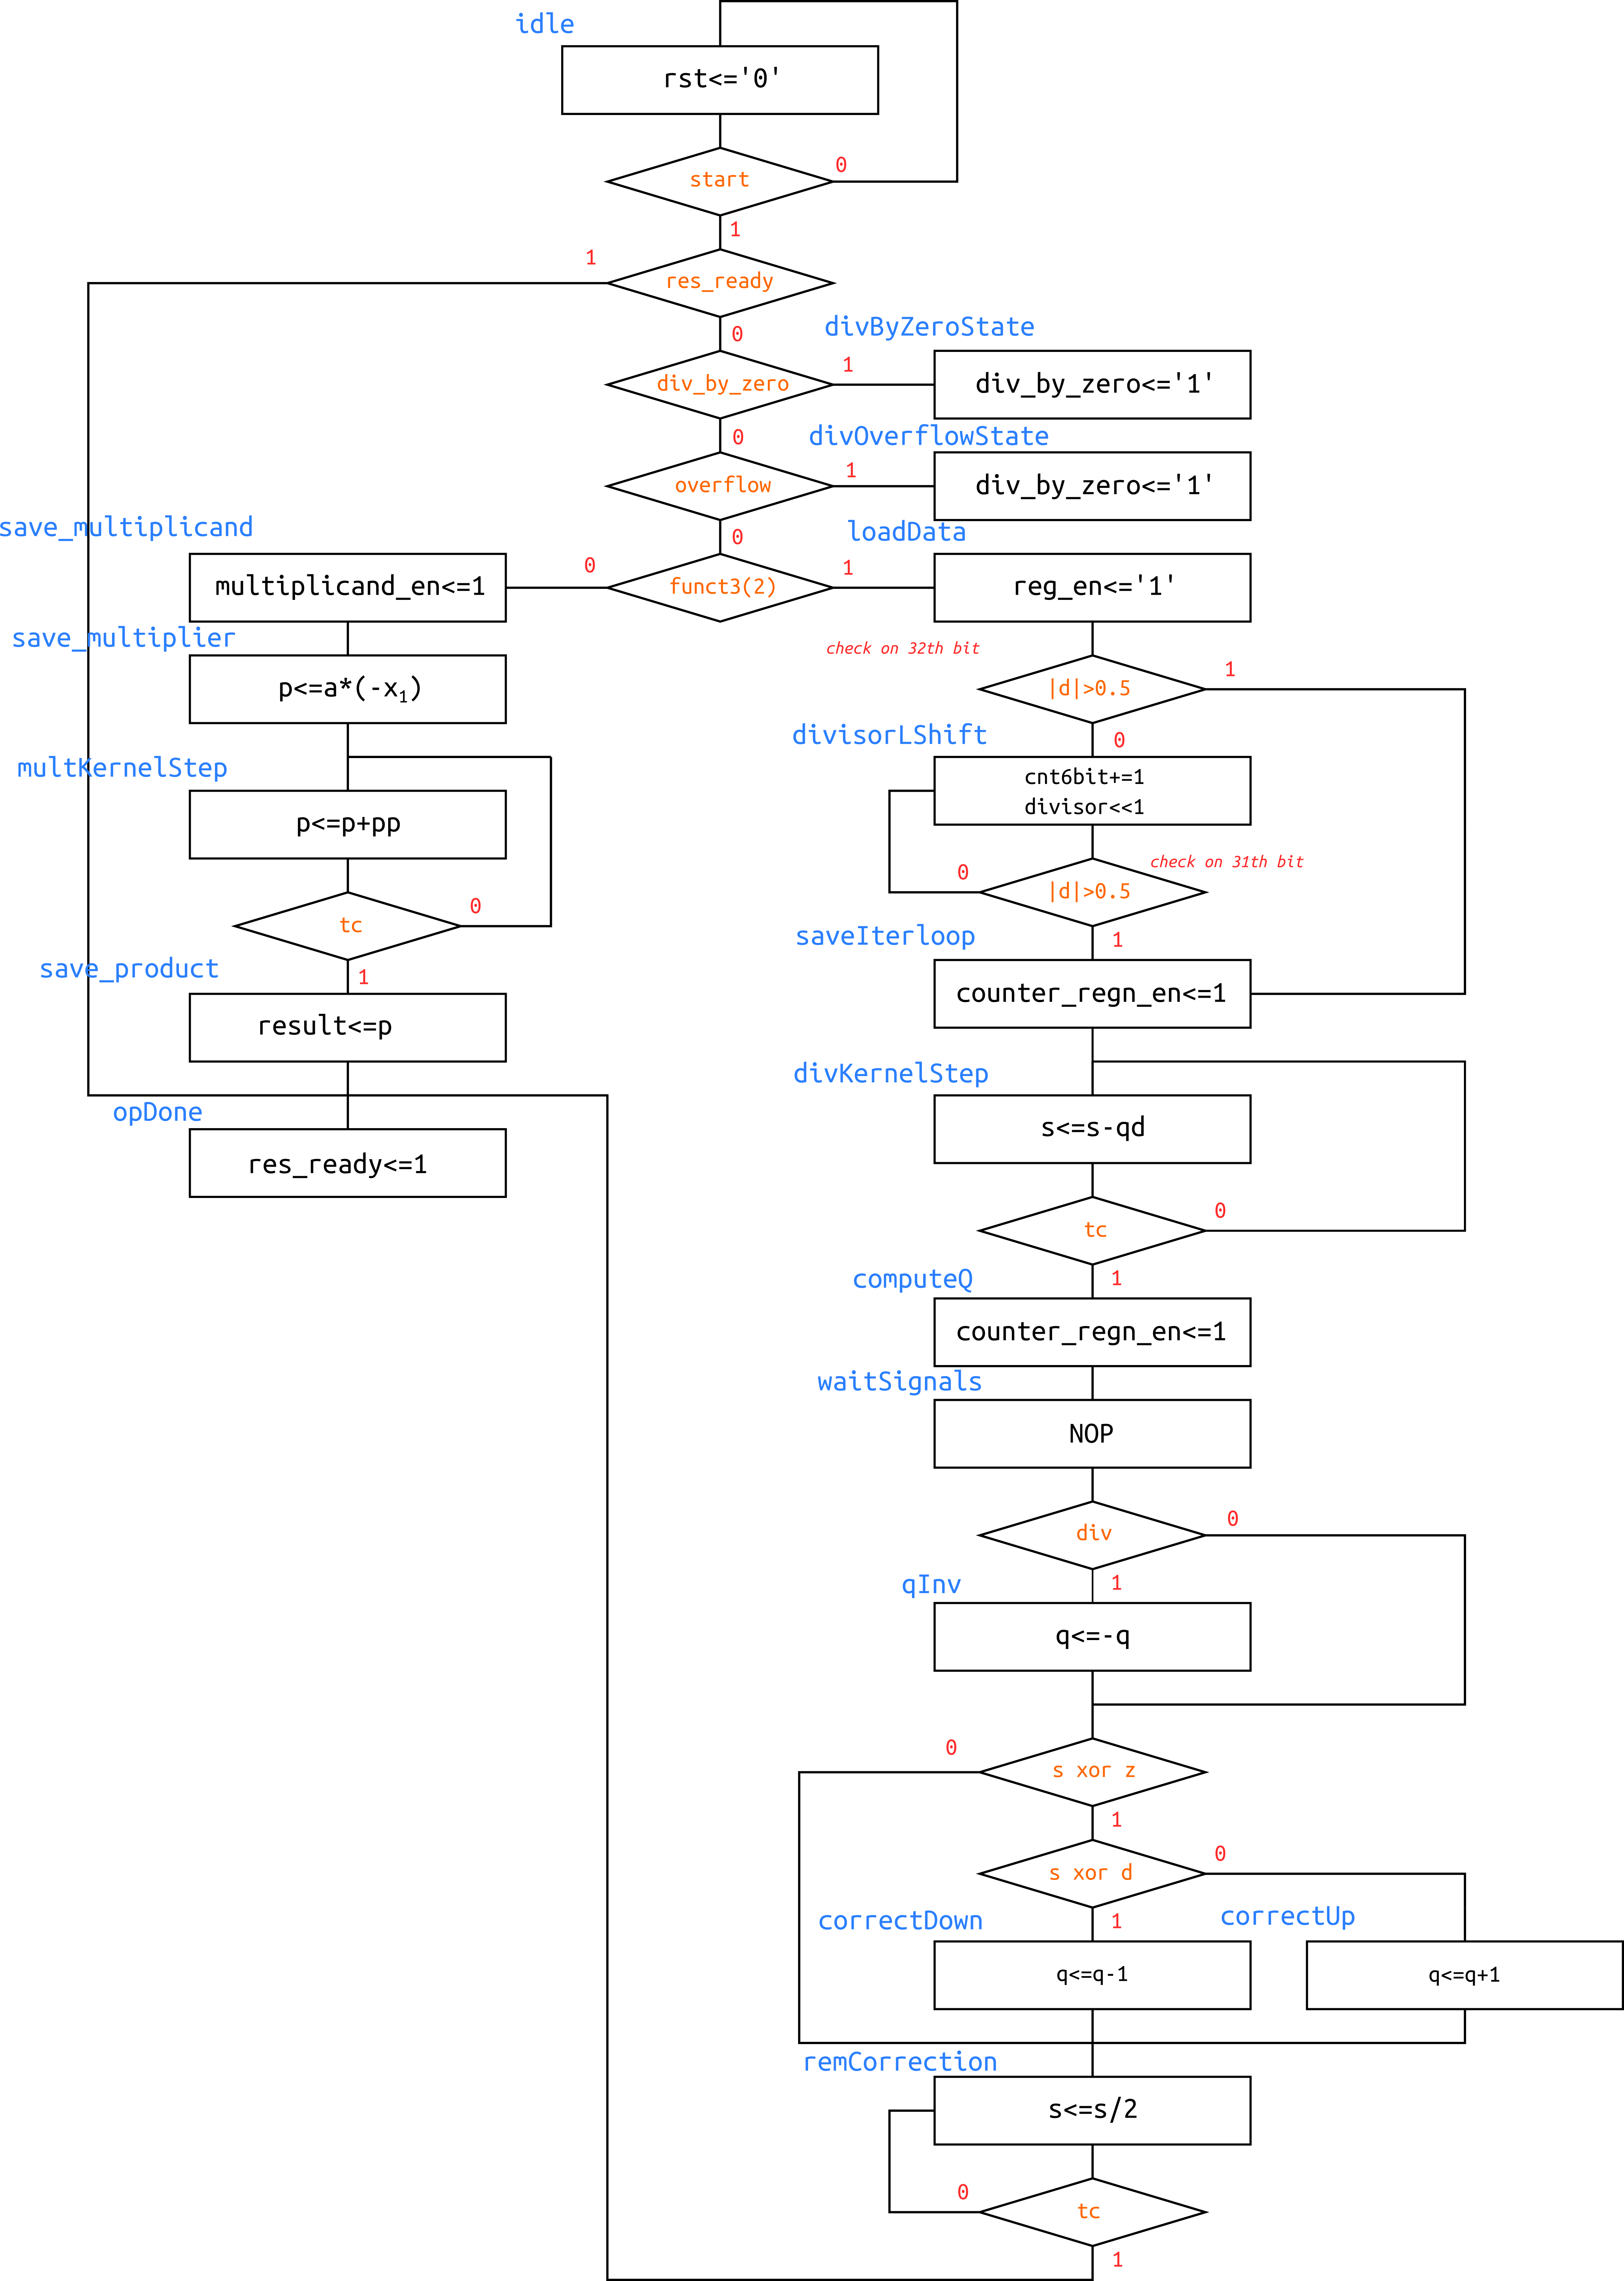
\includegraphics[scale=1]{pics/ASM.png}
    \caption{Complete machine ASM}
    \label{fig:my_label}
\end{figure}
\section{Memory (MEM)}
% overview of the DRAM, the issues with variable latency stalls
The Memory stage of our RISCV Core is mainly composed of the DRAM Controller that handles the DRAM.\newline
We decided to keep things simple in this stage, without replicating the cache structure we adopted in the Fetch Unit, so we opted for a basic combinatory unit that is supposed to write/read into/from the DRAM in the same clock cycle in which the operation is required. The Data RAM, on the other hand, has not been introduced inside the processor core since we assumed it to be an outer (and non synthetizable) module. The controller is capable of correctly handling the sign extension of the operand retrieved from memory in case we've a signed load instruction \textit{lb} or \textit{lh} which load a signed byte or half-word respectively from memory or an unsigned load instruction \textit{lbu} or \textit{lhu}.\newline
An improved version of our core with respect to this stage may implement a similar version of the Instruction Cache, with a \textit{ready} signal to tell the CU when to stall the core in case of a miss; it will also need to handle the data coherency with the main RAM since the content of the two memories may not be the same at any given time instant.

\section{Write Back (WB)}
The Write Back stage is not explicitly reported on the RISCV Core Module and it just consists of the wr\_en signal, the wr\_addr and wr\_data fields that stem from the pipeline registers and go into the related Register File ports in order to allow the writing of the result of the instruction completed.

\chapter{Non-Datapath Logic}
% Here goes anything that is not related to specific a pipeline stage

\section{Branch Prediction Unit}

\section{Branch Forwarding Unit}

\section{Instruction Cache and its Controller}

% add description of bpu

\chapter{Verification and Synthesis}
In order to test our processor core we went through some steps that allowed us to develop a testbench that replicates as much as possible the real situation in which a CPU works.

\section{GCC Toolchain and Test Programs}

\begin{wrapfigure}{R}{.58\textwidth}
\paragraph{}
\vspace*{-\parskip}	\centering
    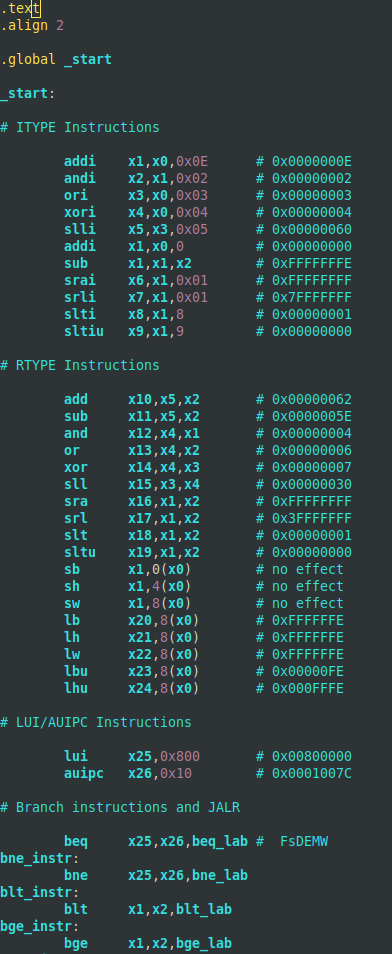
\includegraphics[width=.28\textwidth]{pics/instr_tester1.png}
    %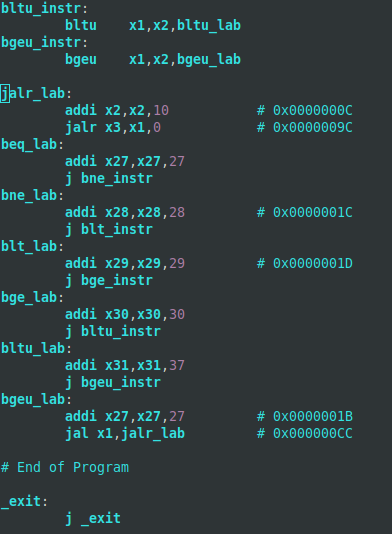
\includegraphics[width=-5\textwidth]{pics/instr_tester2.png}
    \caption{instr\_tester first part}
    \label{fig:instr_tester_1}
\end{wrapfigure}

The first thing we worked on was to find a toolchain that could compile our code into an executable file and then something to convert the executable file into a text file containing the bytes to be loaded into the instruction cache.\newline
In particular, among all the RISCV GCC toolchains that already exist, we were looking for something that would work for bare-metal systems, since we did not want to implement the necessary HW and FW support for OS. What we found was a flexible compiler\footnote{RISCV Toolchain: https://gnu-mcu-eclipse.github.io/toolchain/riscv/} that allows to select the desired architecture and extension in order to determine which subset of instructions to use when compiling the \textit{.c} file. \newline
For our purposes, though, we decided to start from an assembly file in order to check directly whether the instructions work or not. Once the file was compiled using the command \textit{riscv-none-embed-gcc -Wall -nostdlib -march=rv32i -mabi=ilp32 test\_file.s -o test\_file}, we used a basic C program, named \textit{bin2hex.c} in order to convert the executable file into a text file containing all the bytes in which the converted instructions are formed. The text file we obtained in this way is the one that will be loaded into the behavioural IRAM in the same testbench in which the RISCV Core is instantiated.\newline

\begin{wrapfigure}{R}{.58\textwidth}
\paragraph{}
\vspace*{-\parskip}	\centering
    %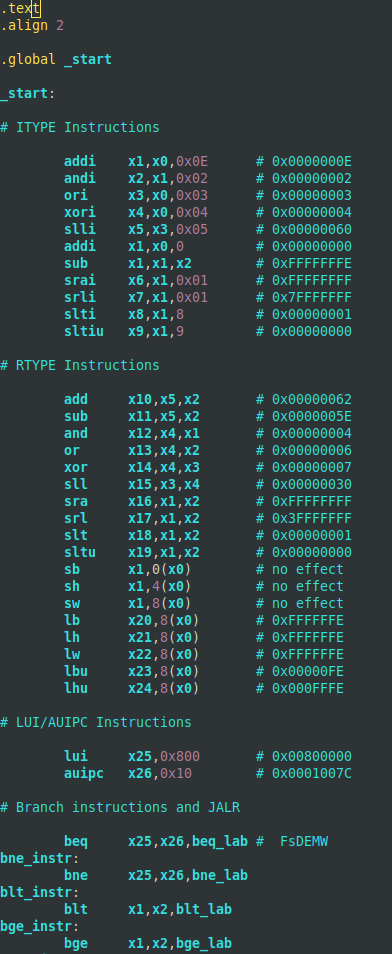
\includegraphics[width=.25\textwidth]{pics/instr_tester1.png}
    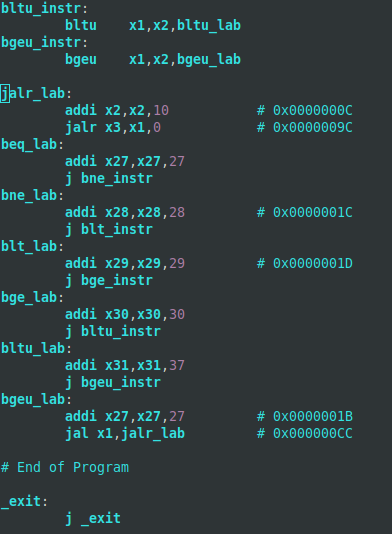
\includegraphics[width=.28\textwidth]{pics/instr_tester2.png}
    \caption{instr\_tester second part}
    \label{fig:instr_tester_2}
\end{wrapfigure}

We wrote two different files to show our core's capabilities: the first one is named \textit{instr\_tester.s} and its purpose is to test every instruction our core can execute in order to test its correct functionality. As we can see in the pictures on the right, first we went through all of the i-type instructions, then the r-type, load, store and lui/auipc instructions and, ultimately, we tried all of the branch and jump instructions. This test was interesting not only because we can make sure almost every submodule and all of their interconnections work correctly, but we could also check the behaviour of the processor when there're instructions in the pipe and the cache has a miss. In fact, since there're many instructions, the cache had a few misses and we were able to see if the processor was able to handle correctly the instructions while fetching the new instruction block from the IRAM.


\newpage
\section{Pre-Synthesis Simulation}


\section{Synthesis}


\section{Post-Synthesis Simulation}

\section{Waveforms}
\section{Automated testing}

\section*{Conclusion}
Our core is wonderful

\end{document}